% !TeX program = xelatex
% Самостоятельный сводный файл. Составлен из tex_результат/1/1.tex ... tex_результат/12/12.tex.
% Материал ответов встроен; \input отдельных ответов не требуется.
\documentclass[12pt,a4paper]{article}
\usepackage{fontspec}
\setmainfont{Times New Roman}
\usepackage[english,russian]{babel}
\usepackage{amsmath,amssymb,mathrsfs,cancel}
\usepackage[margin=22mm]{geometry}
\usepackage{graphicx,float}
\usepackage[unicode,hidelinks]{hyperref}
\DeclareMathOperator{\grad}{grad}
\DeclareMathOperator{\Div}{div}
\newcommand{\Rey}{\mathrm{Re}}
\newcommand{\topic}[1]{\par\medskip\noindent\textbf{#1}\par\nobreak\smallskip}
\newenvironment{textquote}{\begin{quote}\sloppy}{\end{quote}}
\setlength{\emergencystretch}{3em}
\setlength{\parindent}{0pt}
\interfootnotelinepenalty=10000
\sloppy
\newcounter{questionnumber}
\renewcommand{\theHequation}{q\arabic{questionnumber}.\arabic{equation}}
\renewcommand{\thefootnote}{\arabic{footnote})}
\hypersetup{pdftitle={Течения в пористых средах. Вопросы 1–12}}
\begin{document}
\begin{center}
{\LARGE\bfseries Течения в пористых средах\par}
\medskip
{\Large Вопросы 1--12\par}
\end{center}
\noindent К каждому вопросу приведены краткий указатель источников, план рассказа и материал из соответствующего TeX-ответа. Определения, формулы, условия применимости и выводы сохранены из ответов; план служит для навигации. Номера формул относятся к исходным книгам. Отмеченные в ответах неопределённости сохранены.
\tableofcontents

\clearpage
\setcounter{questionnumber}{1}
\setcounter{equation}{0}
\setcounter{footnote}{0}
\phantomsection
\section*{Вопрос 1. Пористая среда и скорость фильтрации}
\addcontentsline{toc}{section}{Вопрос 1. Пористая среда и скорость фильтрации}
\textbf{Формулировка вопроса.} Основные физические сведения о пористых средах. Описание фильтрации в рамках механики сплошных сред. Пористость. Скорость фильтрации.

\medskip
\textbf{Где найти.} Леонтьев, \textit{Основы теории фильтрации}, 2-е изд., 2017; гл. I, §§ 1--2, с. 7--13.

\subsection*{Что рассказать}
\begin{enumerate}
\item Что называют фильтрацией; какие физические факторы вызывают движение жидкости и газа в порах.
\item Переход к механике сплошных сред: осреднение и условие разделения масштабов $d\ll l\ll L$.
\item Пористость, активная пористость и просветность; связь объёмной и площадной характеристик.
\item Скорость фильтрации, её отличие от средней скорости жидкости в порах и выражение расхода через поверхность.
\end{enumerate}
\subsection*{Определения, утверждения, формулы и выводы}
% Исходный ответ: tex_результат/1/1.tex
\begingroup
\newcommand{\source}[2]{\par\nobreak\smallskip{\small Н. Е. Леонтьев. \textit{Основы теории фильтрации}. 2-е изд., 2017. Глава I, §~#1, с.~#2.}\par\medskip}

% Цитата 1; печатные страницы: 7
\begin{textquote}
\textit{Фильтрацией} называется движение (просачивание) жидкостей и газов через пористые среды под действием каких-либо факторов\footnote{Термин «фильтрация» также употребляется в более узком смысле как название процесса очищения жидкости или газа от примесей при течении через фильтр. В англоязычной литературе при описании этих процессов употребляется термин \textit{filtration}, в то время как о фильтрации в широком смысле этого слова говорят обычно как о «течении жидкости через пористую среду» (\textit{flow of a fluid through a porous medium}).}.
\end{textquote}
\source{1}{7}

% Цитата 2; печатные страницы: 7
\begin{textquote}
Вне зависимости от вызывающих фильтрацию причин, которые могут быть совершенно различными --- например, перепад давлений на границе среды, действие внешних массовых сил (сила тяжести, силы инерции, электромагнитные силы) или капиллярных сил на межфазных границах, деформация пористой среды и др.,--- речь всегда идет о движении жидкости по сложной системе разветвленных каналов, сообщающихся между собой. Как правило, внутренняя поверхность порового пространства имеет случайную структуру и не бывает точно известна, поэтому прямое описание движения жидкости во всех подробностях оказывается невозможным.
\end{textquote}
\source{1}{7}

% Цитата 3; печатные страницы: 7--8
\begin{textquote}
К счастью, однако, в большинстве приложений характерные линейные размеры рассматриваемых фильтрационных задач
много больше характерного размера пор, а при практическом изучении фильтрационных явлений обычно интересуются осредненными характеристиками течения. Это позволяет при описании крупномасштабных явлений рассматривать пористый материал как сплошную среду, характеристики которой (плотность и давление жидкости в порах и др.) в каждой точке получаются в результате осреднения по некоторой окрестности, содержащей достаточно большое число пор\footnote{Этот переход вполне аналогичен переходу от молекулярно-кинетической теории к континуальному описанию в случае, когда характерный размер явления много больше длины свободного пробега отдельной молекулы, с той лишь разницей, что в случае фильтрационных явлений описание течений на микроуровне тоже может быть осуществлено в рамках механики сплошных сред.}.
\end{textquote}
\source{1}{7--8}

% Цитата 4; печатные страницы: 8--9
\begin{textquote}
Например, при просачивании воды через пористый пласт под непроницаемой бетонной плотиной (рис.~1) характерный размер пор $d$ (доли миллиметра) много меньше характерного размера пористого пласта $L$ (десятки метров), поэтому мы можем перейти от описания течения на микроуровне (течение внутри конкретной поры) к описанию на макроуровне, считая, что, например, среднее давление $p$ жидкости в порах (в некотором месте внутри пласта в какой-то момент времени) получается осреднением давления в поровом пространстве внутри достаточно малого объема, размеры $l$ которого будут, с одной стороны, много меньше $L$ и, с другой стороны, много больше $d$ (скажем, порядка десятков сантиметров):
\begin{equation}
d\ll l\ll L.
\tag{1.1}\label{q1:eq-1-1}
\end{equation}
При этом, естественно, рассматриваемая величина (в нашем примере давление) будет, вообще говоря, некоторой функцией от
координат и времени: $p=p(x,y,z,t)$.
\end{textquote}
\source{1}{8--9}

% Цитата 5; печатные страницы: 9
\begin{textquote}
Важной характеристикой пористой среды является \textit{пористость} (или \textit{порозность}) $m$, равная относительной объемной доле порового пространства в материале. Пористость определяет количество жидкости, которое может содержаться в некотором объеме пористой среды (если жидкость целиком заполняет внутрипоровое пространство). Если для образца однородного пористого материала объемом $V$ объем пор составляет $V_{\text{п}}$, то пористость этого образца $m=V_{\text{п}}/V$.

Пористость, очевидно, является безразмерной величиной, значения которой лежат в интервале $0<m<1$. Для ориентировки укажем, что пористость почв лежит в диапазоне $0{,}3$--$0{,}7$, речного песка --- $0{,}3$--$0{,}55$, нефтегазоносных пластов, встречающихся на практике, --- $0{,}1$--$0{,}2$.
\end{textquote}
\source{2}{9}

% Цитата 6; печатные страницы: 9
\begin{textquote}
У некоторых пористых материалов часть пор изолирована от остального связного порового пространства или заполнена другой средой (например, при фильтрации воздуха в почве часть пор занята водой, удерживаемой в поровом пространстве за счет капиллярных сил). В подобной ситуации эти поры не участвуют в накоплении и перемещении интересующей нас жидкости внутри пористой среды, и поэтому вместо введенной выше величины (ее называют \textit{полной} или \textit{общей пористостью}) удобно использовать \textit{активную (эффективную) пористость}, равную объемной доле связанных между собой пор, которые могут быть заполнены жидкостью извне. […]
\end{textquote}
\source{2}{9}

% Цитата 7; печатные страницы: 9
\begin{textquote}
Для неоднородных пористых сред, свойства которых могут меняться от точки к точке, пористость $m$ будет некоторой функцией пространственных координат. Если пористая среда может деформироваться (это происходит, например, при утрамбовке грунта или изменении давления в жидкости в порах), то величина пористости может меняться и со временем: $m=m(x,y,z,t)$.
\end{textquote}
\source{2}{9}

% Цитата 8; печатные страницы: 10
\begin{textquote}
Подчеркнем, что при континуальном описании величина пористости (так же как и значения всех остальных осредненных параметров) определяется с помощью осреднения по области с размером порядка $l$, удовлетворяющим \eqref{q1:eq-1-1}.
\end{textquote}
\source{2}{10}

% Цитата 9; печатные страницы: 10
\begin{textquote}
Если сделать мысленный поперечный разрез образца пористой среды, то в образовавшемся сечении (обозначим его площадь $S$) часть площади $S_{\text{п}}$ будет приходиться на поры, а оставшаяся часть $S-S_{\text{п}}$ --- на твердое вещество пористой среды\footnote{«Каркас» пористой среды часто называют \textit{пористым скелетом} или \textit{матрицей}. Отметим также, что в отношении фильтрующейся среды (жидкой или газообразной) иногда применяется термин \textit{флюид}.}. Отношение $n$ площади пор в сечении к общей площади сечения называется \textit{просветностью (поверхностной пористостью)}: $n=S_{\text{п}}/S$.
\end{textquote}
\source{2}{10}

% Цитата 10; печатные страницы: 10--11
\begin{textquote}
Величина просветности зависит от того, через какую точку и в каком направлении проводится разрез среды, однако, что замечательно, \textit{среднее значение просветности} для большого набора параллельных сечений какого-то фиксированного образца равно
пористости этого образца.

[…]

Доказанное свойство позволяет приближенно считать пористость и просветность равными величинами для реальных пористых сред со случайной структурой: $m\approx n$.
\end{textquote}
\source{2}{10--11}

% Цитата 11; печатные страницы: 11
\begin{textquote}
Обратим внимание, что упоминавшиеся выше геометрические по своей природе параметры (пористость, характерный размер пор, функция распределения пор по радиусам) в общем случае не характеризуют полностью способность пористой среды пропускать через себя жидкость. Например, проницаемую для жидкости пористую среду можно превратить в непроницаемую, если ввести внутри порового пространства некоторое количество тонких перегородок, которые практически не поменяют перечисленные средние характеристики, но существенно изменят проводимость среды.
\end{textquote}
\source{2}{11}

% Цитата 12; печатные страницы: 11--12
\begin{textquote}
Для характеристики массопереноса при фильтрации жидкости (или газа) вводится векторная величина, называемая \textit{скоростью фильтрации}. Рассмотрим сначала простейший случай, когда жидкость движется вдоль тонкой прямолинейной трубки, заполненной пористым материалом. Для такого течения скорость фильтрации определяется как вектор $\boldsymbol{u}$, направленный в сторону движения
жидкости, величина которого равна объемному расходу жидкости (объему жидкости, протекающей в единицу времени) в расчете на единицу площади \textit{полного поперечного сечения} трубки (включающего как поры, так и пористую среду).

Здесь важно подчеркнуть, что хотя скорость фильтрации имеет размерность скорости, она тем не менее не равна скорости движения отдельных частиц жидкости. Действительно, если $S$ --- площадь поперечного сечения трубки, $S_{\text{п}}$ --- часть площади этого сечения, приходящаяся на поры, то постоянство объемного расхода однородной несжимаемой жидкости можно записать в виде
\[
Q=|\boldsymbol{u}|S=vS_{\text{п}}=\mathrm{const},
\]
где $Q$ --- объемный расход жидкости через трубку, $v$ --- среднее значение проекции \textit{скорости частиц жидкости} на ось трубки, вычисленное по площади сечения, занимаемой порами. Отсюда получаем
\[
v=\frac{|\boldsymbol{u}|S}{S_{\text{п}}}=\frac{|\boldsymbol{u}|}{n}\approx\frac{|\boldsymbol{u}|}{m},
\]
т.е. средняя скорость частиц жидкости приблизительно в $1/m$ раз больше скорости фильтрации.
\end{textquote}
\source{2}{11--12}

% Цитата 13; печатные страницы: 12
\begin{textquote}
В общем случае неодномерного движения жидкости в пористой среде \textit{скорость фильтрации} определяется как вектор $\boldsymbol{u}$, проекция которого на некоторое направление равна объемному расходу жидкости через единичную площадку, перпендикулярную данному направлению. С помощью этого определения легко вычисляются объемный расход $Q$ и массовый расход $Q_{\text{м}}$ жидкости через произвольную поверхность $\Sigma$, проведенную внутри пористой среды:
\begin{equation}
Q=\int_{\Sigma}\boldsymbol{u}\cdot\boldsymbol{n}\,d\sigma,
\qquad Q_{\text{м}}=\int_{\Sigma}\rho\boldsymbol{u}\cdot\boldsymbol{n}\,d\sigma,
\tag{2.1}\label{q1:eq-2-1}
\end{equation}
где $\rho=\rho(x,y,z,t)$ --- плотность фильтрующейся жидкости, $\boldsymbol{n}$ --- вектор нормали к поверхности $\Sigma$.

Удобство использования скорости фильтрации при практических исследованиях состоит в том, что с ее помощью можно находить расход жидкости без использования информации о пористости, которая явно не входит в соотношения \eqref{q1:eq-2-1}.
\end{textquote}
\source{2}{12}
\endgroup

\clearpage
\setcounter{questionnumber}{2}
\setcounter{equation}{0}
\setcounter{footnote}{0}
\phantomsection
\section*{Вопрос 2. Закон Дарси и его обобщения}
\addcontentsline{toc}{section}{Вопрос 2. Закон Дарси и его обобщения}
\textbf{Формулировка вопроса.} Закон Дарси и пределы его применимости. Учёт анизотропии пористой среды. Двучленный закон фильтрации Форхгеймера. Фильтрация с предельным градиентом давления.

\medskip
\textbf{Где найти.} Леонтьев, 2017; гл. I, §§ 3--4, с. 13--24.

\subsection*{Что рассказать}
\begin{enumerate}
\item Закон Дарси с массовыми силами; физический смысл проницаемости и коэффициента фильтрации.
\item Тензор проницаемости анизотропной среды; возможное несовпадение направлений скорости и градиента давления.
\item Область применимости линейного закона, роль числа Рейнольдса и двучленный закон Форхгеймера.
\item Закон с предельным градиентом: условие отсутствия движения и физическая модель вязкопластической жидкости.
\end{enumerate}
\subsection*{Определения, утверждения, формулы и выводы}
% Исходный ответ: tex_результат/2/2.tex
\begingroup
\newcommand{\source}[2]{\par\nobreak\smallskip{\small Н. Е. Леонтьев. \textit{Основы теории фильтрации}. 2-е изд., 2017. Глава I, §~#1, с.~#2.}\par\medskip}

% Цитата 1; печатные страницы: 14--15
\begin{textquote}
Исторически уравнение баланса импульса было экспериментально получено французским гидравликом Анр\'и Дарс\'и (H.Darcy, 1856) для случая медленного стационарного движения несжимаемой жидкости в неподвижной изотропной пористой
среде. В современных обозначениях это соотношение, называемое \textit{законом Дарси}, для фильтрации в поле тяжести имеет вид
\begin{equation}
0=-\grad p+\rho\boldsymbol{g}-\frac{\mu}{k}\boldsymbol{u},
\tag{3.3}\label{q2:eq-3-3}
\end{equation}
где $\boldsymbol{g}$ --- ускорение свободного падения, $\mu$ --- коэффициент динамической вязкости жидкости, $k$ --- коэффициент, называемый проницаемостью пористой среды, который зависит от типа пористой среды. По структуре уравнение \eqref{q2:eq-3-3} похоже на уравнение Навье--Стокса для вязкой несжимаемой жидкости при $\mu=\mathrm{const}$:
\begin{equation}
\rho\frac{d\boldsymbol{v}}{dt}=-\grad p+\rho\boldsymbol{g}+\mu\triangle\boldsymbol{v}
\tag{3.4}\label{q2:eq-3-4}
\end{equation}
и это не удивительно: макроскопический закон движения при фильтрации в пористой среде (закон Дарси) может быть получен с помощью некоторой процедуры осреднения из уравнения движения, описывающего внутрипоровое движение жидкости на микроуровне, то есть уравнения Навье--Стокса (см. § 5).
\source{3}{14--15}
\end{textquote}

% Цитата 2; печатные страницы: 15
\begin{textquote}
При медленных (ползущих) течениях внутри пористой среды, для которых и справедлив закон Дарси, инерционные силы много меньше вязких сил, поэтому сто\'ящим в левой части \eqref{q2:eq-3-4} ускорением можно пренебречь, что даст при осреднении ноль в левой части \eqref{q2:eq-3-3}. Наличие же последнего слагаемого в \eqref{q2:eq-3-4}, описывающего действие вязкости, приводит при переходе к макроскопическому описанию к появлению объемной силы вязкого сопротивления, действующей на жидкость со стороны пористого скелета. В рассматриваемом случае медленных течений\footnote[1]{Более точно --- при числах Рейнольдса $\Rey=\rho vd/\mu\ll1$.} в изотропной среде сила сопротивления направлена противоположно скорости фильтрации, а ее величина прямо пропорциональна вязкости и модулю скорости фильтрации.
\source{3}{15}
\end{textquote}

% Цитата 3; печатные страницы: 15
\begin{textquote}
При $\boldsymbol{g}=0$ закон Дарси приобретает вид
\begin{equation}
\boldsymbol{u}=-\frac{k}{\mu}\grad p;
\tag{3.5}\label{q2:eq-3-5}
\end{equation}
знак минус в правой части \eqref{q2:eq-3-5} имеет ясный физический смысл: в отсутствие массовых сил жидкость движется в пористой среде из областей с б\'ольшим давлением в области с меньшим давлением.
\source{3}{15}
\end{textquote}

% Цитата 4; печатные страницы: 16
\begin{textquote}
Коэффициент проницаемости $k$ зависит только от свойств пористой среды (но не от свойств жидкости), и определяется, в основном, геометрией порового пространства.

[…]

Для неоднородных пористых сред коэффициент проницаемости является функцией пространственных координат и может меняться с течением времени (например, при деформациях пористого скелета или за счет его засорения или растворения).
\source{3}{16}
\end{textquote}

% Цитата 5; печатные страницы: 17
\begin{textquote}
При фильтрации в анизотропных пористых средах (например, в осадочных слоистых пластах или в средах с трещинами, направленными в выделенном направлении) линейная зависимость скорости фильтрации и градиента давления сохраняется (для медленных течений), однако эти векторы в случае общего положения уже не будут параллельны. Проницаемость таких сред будет характеризоваться не одним числом (коэффициентом проницаемости $k$), а симметричным положительно-определенным \textit{тензором проницаемости} $k_{ij}$, входящим в закон Дарси
\[
u_i=-\frac{k_{ij}}{\mu}(\nabla^jp-\rho g^j).
\]
Например, в слоистой среде, у которой направление, перпендикулярное плоскости напластования, задается единичным вектором $\boldsymbol{n}$, тензор проницаемости в декартовой системе координат имеет вид
\[
k_{ij}=(k_\perp-k_\parallel)n_in_j+k_\parallel\delta_{ij},
\]
где $k_\perp$ и $k_\parallel$ суть проницаемости при фильтрации соответственно поперек и вдоль напластования.
\source{3}{17}
\end{textquote}

% Цитата 6; печатные страницы: 18
\begin{textquote}
В некоторых практически важных ситуациях при фильтрации жидкостей --- речь идет об однородных жидкостях, целиком заполняющих недеформируемые изотропные пористые среды --- наблюдаются отступления от классического закона Дарси \eqref{q2:eq-3-3}. Эти отклонения связаны с двумя причинами. \textit{Первая} --- это немалость скоростей движения жидкости внутри пор, т.е. невозможность пренебречь инерционными членами в микроскопических уравнениях \eqref{q2:eq-3-4}. Такие условия, в которых неприменимо приближение Стокса, возникают, например, в прискважинных областях или при фильтрации в крупнозернистых пористых средах (фильтрация через гравий и гальку, а также через гранулированные среды в промышленных технологических установках). \textit{Вторая} причина состоит в отличии реологических\footnote[1]{Реология --- наука, изучающая связи между напряжениями и деформационными характеристиками материалов. Название науки, предложенное американским исследователем Ю.Бингамом (E.Bingham, 1920), происходит от греческого $\rho\varepsilon\omega$ --- «теку», «струюсь».} соотношений фильтрующейся жидкости от закона Навье--Стокса, причем неньютоновское поведение жидкостей при течении внутри порового пространства может проявляться как в узкой пристеночной области (за счет физико-химического взаимодействия жидкости со стенкой поры), так и во всем объеме жидкости (например, при фильтрации некоторых нефтей).
\source{4}{18}
\end{textquote}

% Цитата 7; печатные страницы: 18--19
\begin{textquote}
Предполагая для простоты, что массовые силы отсутствуют\footnote[2]{Влияние потенциальных сил можно учесть путем переопределения давления (например, в случае фильтрации несжимаемой однородной жидкости в поле силы тяжести --- с помощью введения новой переменной $p'=p-\rho\boldsymbol{r}\cdot\boldsymbol{g}$, где $\boldsymbol{r}$ --- радиус-вектор).}, установим общий вид зависимости градиента давления от скорости фильтрации с использованием теории размерностей.

Модуль градиента давления $|\grad p|$ при стационарной фильтрации зависит, кроме модуля скорости фильтрации $u$, от свойств жидкости (плотности $\rho$ и вязкости $\mu$) и пористой среды (характерного размера пор $d$, пористости $m$ и, возможно, других скалярных безразмерных параметров $a_\alpha$, определяющих геометрию
порового пространства):
\[
|\grad p|=F(u,\rho,\mu,d,m,a_\alpha),
\]
и применение $\pi$-теоремы [6,15] дает зависимость
\[
|\grad p|=\frac{\mu u}{d^2}\cdot\Phi(\Rey,m,a_\alpha),\qquad \Rey=\frac{\rho ud}{\mu}.
\]
\source{4}{18--19}
\end{textquote}

% Цитата 8; печатные страницы: 19--20
\begin{textquote}
Итак, общий вид закона фильтрации несжимаемой жидкости в изотропной пористой среде можно записать так:
\begin{equation}
\grad p=-\frac{\mu\boldsymbol{u}}{d^2}\Phi(\Rey,m,a_\alpha).
\tag{4.1}\label{q2:eq-4-1}
\end{equation}
Зависимость $\Phi(\Rey)$ в двух предельных случаях --- при малых и больших числах Рейнольдса --- можно установить из общих соображений.

В случае \textit{очень медленных} (ползущих) внутрипоровых течений, в которых доминируют вязкие эффекты, зависимость \eqref{q2:eq-4-1}
не должна содержать плотность жидкости, выпадающую из уравнений вязкой жидкости в приближении Стокса. Поэтому при $\Rey\ll1$ функция $\Phi$ не должна зависеть от числа Рейнольдса, и закон фильтрации \eqref{q2:eq-4-1} можно записать в виде
\[
\grad p=-\frac{\mu}{k}\boldsymbol{u},\quad k=\frac{d^2}{\Phi(0,m,a_\alpha)},
\]
где величина $k$, имеющая размерность квадрата длины и зависящая только от свойств пористой среды, должна, в силу закона Дарси \eqref{q2:eq-3-5}, совпадать с коэффициентом проницаемости.
\source{4}{19--20}
\end{textquote}

% Цитата 9; печатные страницы: 20
\begin{textquote}
В противоположном случае \textit{быстрых внутрипоровых течений} (при $\Rey\gg1$) преобладающими должны быть инерционные эффекты, поэтому зависимость градиента давления от скорости фильтрации не должна содержать в главных членах коэффициент вязкости $\mu$. Это дает при больших $\Rey$ линейную зависимость $\Phi(\Rey)$ и квадратичную зависимость $|\grad p|$ от $u$.

Если нормировать функцию $\Phi(\Rey)$, вводя обозначение
\begin{equation}
f(\Rey)=\Phi(\Rey)/\Phi(0),\quad f(0)=1,\quad f(\Rey)=O(\Rey)\text{ при }\Rey\to\infty,
\tag{4.2}\label{q2:eq-4-2}
\end{equation}
то закон фильтрации в принимает окончательный вид
\[
0=-\grad p+\rho\boldsymbol{g}-\frac{\mu}{k}\boldsymbol{u}\cdot f(\Rey),\quad \Rey=\frac{\rho ud}{\mu}.
\]
\source{4}{20}
\end{textquote}

% Цитата 10; печатные страницы: 21
\begin{textquote}
При практических расчетах закон $f(\Rey)$ часто аппроксимируют линейной зависимостью, удовлетворяющей требованиям \eqref{q2:eq-4-2}:
\[
f(\Rey)=1+\frac{\beta\sqrt{k}}{d}\Rey,
\]
где $\beta$ --- безразмерный параметр, зависящий от структуры пористой среды (порядка единицы). Это дает \textit{двучленный закон фильтрации}, называемый также \textit{законом фильтрации Форхгеймера} (P.Forchheimer, 1901):
\begin{equation}
0=-\grad p+\rho\boldsymbol{g}-\frac{\mu}{k}\boldsymbol{u}-\beta\frac{\rho u^2}{\sqrt{k}}\cdot\frac{\boldsymbol{u}}{u}.
\tag{4.3}\label{q2:eq-4-3}
\end{equation}
\source{4}{21}
\end{textquote}

% Цитата 11; печатные страницы: 21
\begin{textquote}
Как видно из рис.~5, отклонения от закона Дарси, которому соответствует горизонтальный участок графика, начинаются при $\Rey$ порядка единиц (числа Рейнольдса вычисляются по характерному размеру зерен). При дальнейшем повышении скорости фильтрации инерцией жидкости при ее движении в извилистом внутрипоровом пространстве уже нельзя пренебрегать и нужно пользоваться, например, квадратичной зависимостью \eqref{q2:eq-4-3}. Этот закон по своей структуре (квадратичная зависимость от скорости) похож на известную связь сопротивления и скорости при развитом турбулентном движении жидкости в каналах или при обтекании тел потоком. Основываясь на этой формальной аналогии, иногда режим фильтрации в области применимости закона \eqref{q2:eq-4-3} называют «турбулентной фильтрацией». В действительности же, как показывают эксперименты, при переходе через границу применимости закона Дарси движение жидкости в порах остается ламинарным, а переход к турбулентности происходит при достаточно больших числах Рейнольдса (около 100--300).
\source{4}{21}
\end{textquote}

% Цитата 12; печатные страницы: 22--23
\begin{textquote}
В ряде природных процессов, например при просачивании воды в мелкопористых средах или при фильтрации некоторых нефтей, течение жидкости начинается при превышении модулем градиента давления $|\grad p|$ некоторого фиксированного порогового
значения $G$ («предельного градиента»), а при меньших градиентах жидкость в порах покоится\footnote[1]{Отметим для сравнения, что при выполнении закона Дарси фильтрационное течение начинается при любых сколь угодно малых градиентах давления.}.
\source{4}{22--23}
\end{textquote}

% Цитата 13; печатные страницы: 23
\begin{textquote}
Для моделирования таких явлений часто используется \textit{закон фильтрации с предельным (начальным) градиентом}
\begin{equation}
\boldsymbol{u}=\begin{cases}
-\dfrac{k}{\mu}(|\grad p|-G)\cdot\dfrac{\grad p}{|\grad p|}&\text{при }|\grad p|\geqslant G,\\[6pt]
0&\text{при }|\grad p|<G.
\end{cases}
\tag{4.4}\label{q2:eq-4-4}
\end{equation}
Особенностью этой модели является возможность существования застойных зон (с нулевой скоростью фильтрации), в которых давление не определено однозначно и зависит от предыстории течения.
\source{4}{23}
\end{textquote}

% Цитата 14; печатные страницы: 23--24
\begin{textquote}
Наличие предельного градиента легко объяснить, если предположить, что фильтрующаяся жидкость проявляет \textit{вязкопластические свойства} (т.е. начинает течь лишь тогда, когда интенсивность касательных напряжений --- функция от второго инварианта девиатора тензора напряжений --- достигает фиксированного ненулевого значения). Например, жидкость Бингама--Шведова,
которая при простом сдвиге описывается соотношениями
\[
e_{xy}=\begin{cases}
\dfrac{1}{2\mu}(|\tau_{xy}|-\tau_0)\cdot\dfrac{\tau_{xy}}{|\tau_{xy}|}&\text{при }|\tau_{xy}|\geqslant\tau_0,\\[6pt]
0&\text{при }|\tau_{xy}|<\tau_0,
\end{cases}
\]
начинает движение в цилиндрическом капилляре радиуса $R$ при превышении градиентом давления значения $|\grad p|=2\tau_0/R$ ($\tau_0$ --- пороговое касательное напряжение)\footnote[1]{Уточним, что в движение приходит пристеночный слой жидкости; в центральной части капилляра при любых, даже очень больших градиентах некоторая часть жидкости движется как твердое тело.}. При моделировании пористой среды набором параллельных каналов с различными радиусами отсюда получается закон фильтрации, качественно схожий с \eqref{q2:eq-4-4}, причем предельный градиент определяется радиусом наибольшего капилляра.
\source{4}{23--24}
\end{textquote}
\endgroup

\clearpage
\setcounter{questionnumber}{3}
\setcounter{equation}{0}
\setcounter{footnote}{0}
\phantomsection
\section*{Вопрос 3. Балансы, разрывы и граничные условия}
\addcontentsline{toc}{section}{Вопрос 3. Балансы, разрывы и граничные условия}
\textbf{Формулировка вопроса.} Уравнения баланса массы, импульса и энергии для течений в пористых средах. Соотношения на разрывах. Типичные граничные условия.

\medskip
\textbf{Где найти.} Леонтьев, 2017; гл. I, §§ 3, 5--6, с. 13--17, 24--37.

\subsection*{Что рассказать}
\begin{enumerate}
\item Интегральный и локальный баланс массы; закон Дарси и осреднённое уравнение движения.
\item Условия осреднения, сила сопротивления и связь микроскопических и макроскопических величин.
\item Баланс энергии и дополнительные предположения, позволяющие упростить его.
\item Соотношения на разрывах из интегральных законов; условия на непроницаемой стенке, свободной поверхности и границе пористых сред.
\end{enumerate}
\subsection*{Определения, утверждения, формулы и выводы}
% Исходный ответ: tex_результат/3/3.tex
\begingroup
\newcommand{\source}[2]{\par\nobreak\smallskip{\small Н. Е. Леонтьев. \textit{Основы теории фильтрации}. 2-е изд., 2017. Глава I, §~#1, с.~#2.}\par\medskip}

% Цитата 1; печатные страницы: 14
\begin{textquote}
Интегральная формулировка закона сохранения массы жидкости получается из утверждения о том, что изменение массы жидкости в произвольном объеме $V$ внутри пористой среды происходит за счет притока жидкости через границу объема $\Sigma$:
\[
\frac{d}{dt}\int_V\rho m\,dV=-\int_\Sigma\rho\boldsymbol{u}\cdot\boldsymbol{n}\,d\sigma.
\]
Здесь $\boldsymbol{n}$ --- вектор внешней нормали к поверхности $\Sigma$ (из-за такого выбора нормали интеграл в правой части стоит со знаком минус), а объем $V$ неподвижен относительно пористой среды. Если входящие в это уравнение функции являются достаточно гладкими, то в левой части можно занести производную под знак интеграла, а правую часть преобразовать с помощью теоремы Гаусса--Остроградского:
\[
\int_V\frac{\partial(\rho m)}{\partial t}\,dV=-\int_V\Div(\rho\boldsymbol{u})\,dV,
\]
откуда в силу произвольности объема $V$ получается дифференциальная запись закона сохранения массы --- \textit{уравнение неразрывности}:
\begin{equation}
\frac{\partial(\rho m)}{\partial t}+\Div(\rho\boldsymbol{u})=0.
\tag{3.1}\label{q3:eq-3-1}
\end{equation}
Если плотность жидкости постоянна, а пористая среда не деформируется (т.е. пористость зависит только от координат), то первое слагаемое обращается в ноль и уравнение неразрывности приобретает вид
\begin{equation}
\Div\boldsymbol{u}=0.
\tag{3.2}\label{q3:eq-3-2}
\end{equation}
\source{3}{14}
\end{textquote}

% Цитата 2; печатные страницы: 14--15
\begin{textquote}
Исторически уравнение баланса импульса было экспериментально получено французским гидравликом Анр\'и Дарс\'и (H.Darcy, 1856) для случая медленного стационарного движения несжимаемой жидкости в неподвижной изотропной пористой
среде. В современных обозначениях это соотношение, называемое \textit{законом Дарси}, для фильтрации в поле тяжести имеет вид
\begin{equation}
0=-\grad p+\rho\boldsymbol{g}-\frac{\mu}{k}\boldsymbol{u},
\tag{3.3}\label{q3:eq-3-3}
\end{equation}
где $\boldsymbol{g}$ --- ускорение свободного падения, $\mu$ --- коэффициент динамической вязкости жидкости, $k$ --- коэффициент, называемый проницаемостью пористой среды, который зависит от типа пористой среды.
\source{3}{14--15}
\end{textquote}

% Цитата 3; печатные страницы: 25
\begin{textquote}
В случае \textit{недеформируемого неподвижного} пористого скелета, которым мы для простоты ограничимся, при вычислении среднего от производных справедливы равенства
\begin{equation}
\left\langle\frac{\partial A}{\partial t}\right\rangle=\frac{\partial\langle A\rangle}{\partial t},\qquad
\left\langle\frac{\partial A}{\partial x^i}\right\rangle=\frac{\partial\langle A\rangle}{\partial x^i}+\frac{1}{|V|}\int_{\Sigma_{\text{ж-с}}}An_i\,d\sigma,
\tag{5.1}\label{q3:eq-5-1}
\end{equation}
где $\Sigma_{\text{ж-с}}$ --- граница жидкости и скелета, попадающая внутрь $V$, $\boldsymbol{n}=(n_x;n_y;n_z)$ --- вектор внешней нормали к заштрихованному на рис.~7 объему $V_{\text{ж}}$ жидкости, находящейся внутри сферы.
\source{5}{25}
\end{textquote}

% Цитата 4; печатные страницы: 26--27
\begin{textquote}
Теперь с помощью (5.1) несложно получить осредненные уравнения фильтрации. Проделаем это для случая однородной \textit{несжимаемой} ньютоновской жидкости.

\topic{Осреднение микроскопического уравнения неразрывности}
Осреднение уравнения неразрывности $\Div\boldsymbol{v}=0$ производится очень просто:
\[
\langle\nabla_iv^i\rangle=\nabla_i\langle v^i\rangle+\frac{1}{|V|}\int_{\Sigma_{\text{ж-с}}}v^in_i\,d\sigma=0,
\]
откуда с учетом условия прилипания получаем выражение закона сохранения массы в терминах средних параметров:
\begin{equation}
\nabla_i\langle v^i\rangle\equiv\Div\langle\boldsymbol{v}\rangle=0.
\tag{5.2}\label{q3:eq-5-2}
\end{equation}
Величина, стоящая под знаком дивергенции, есть не что иное, как скорость фильтрации:
\[
\langle\boldsymbol{v}\rangle=\boldsymbol{u},
\]
так что (5.2) совпадает с (3.2).

\topic{Осреднение микроскопического уравнения движения}
Для осреднения удобно взять уравнение движения в дивергентном виде
\[
\rho\left(\frac{\partial v^i}{\partial t}+\nabla_k(v^kv^i)\right)=\nabla_kp^{ik}+\rho F^i,
\]
в котором $p^{ik}$ --- компоненты тензора напряжений, $F^i$ --- компоненты вектора массовой плотности внешних объемных сил. Применяя (5.1) и учитывая условие прилипания, получим
\[
\rho\left(\frac{\partial\langle v^i\rangle}{\partial t}+\nabla_k\langle v^kv^i\rangle\right)=\nabla_k\langle p^{ik}\rangle+F^i_{\text{с-ж}}+\rho\langle F^i\rangle,
\]
\[
F^i_{\text{с-ж}}=\frac{1}{|V|}\int_{\Sigma_{\text{ж-с}}}p^{ik}n_k\,d\sigma,
\]
где сила $\boldsymbol{F}_{\text{с-ж}}$, вид которой будет обсуждаться чуть позже, представляет собой \textit{полную} силу (в расчете на единицу объема), действующую со стороны скелета на жидкость внутри объема $V$, т.е. включает в себя как результат действия вязких касательных напряжений, так и результат суммирования нормальных напряжений на границе жидкости и скелета. Первое слагаемое в правой части, снова с учетом условия прилипания, принимает вид
\[
\begin{aligned}
\nabla_k\langle p^{ik}\rangle
&=\nabla_k\left\langle-pg^{ik}+\mu(\nabla^iv^k+\nabla^kv^i)\right\rangle=\\
&=-\nabla^i\langle p\rangle+\cancel{\mu\nabla_k\nabla^i\langle v^k\rangle}+\mu\nabla_k\nabla^k\langle v^i\rangle,
\end{aligned}
\]
где зачеркнутый член пропадает вследствие (5.2), что в результате дает
\begin{equation}
\begin{aligned}
\rho\left(\frac{\partial\langle v^i\rangle}{\partial t}+\nabla_k\langle v^kv^i\rangle\right)
&=-\nabla^i\langle p\rangle+\mu\triangle\langle v^i\rangle\\
&\quad+\rho\langle F^i\rangle+F^i_{\text{с-ж}}.
\end{aligned}
\tag{5.3}\label{q3:eq-5-3}
\end{equation}
Уравнение (5.3) является точным, и дальнейшее его упрощение связанно с дополнительными гипотезами и оценкой входящих в него членов.
\source{5}{26--27}
\end{textquote}

% Цитата 5; печатные страницы: 28
\begin{textquote}
Удобно выделить в явном виде \textit{силу сопротивления} (в расчете \textit{на единицу объема жидкости}), связанную --- прямо или косвенно --- с действием вязких сил и обращающуюся в ноль при $\boldsymbol{u}=0$, и переписать уравнение движения в виде
\begin{equation}
\begin{gathered}
0=-\grad p+\rho\boldsymbol{F}+\boldsymbol{F}_{\text{сопр}},\\
\boldsymbol{F}_{\text{сопр}}=\frac{1}{m}(\boldsymbol{F}_{\text{с-ж}}-p\grad m).
\end{gathered}
\tag{5.4}\label{q3:eq-5-4}
\end{equation}
\source{5}{28}
\end{textquote}

% Цитата 6; печатные страницы: 29
\begin{textquote}
В случае постоянной пористости закон (5.4) должен совпадать с законом Дарси, поэтому сила сопротивления
\[
\boldsymbol{F}_{\text{сопр}}=\frac{1}{m}\boldsymbol{F}_{\text{с-ж}}=-\frac{\mu}{k}\boldsymbol{u}.
\]
\source{5}{29}
\end{textquote}

% Цитата 7; печатные страницы: 29--30
\begin{textquote}
Осреднение уравнения энергии для жидкости
\[
\begin{aligned}
\frac{\partial}{\partial t}\left(\rho\left(U+\frac{v^2}{2}\right)\right)
&+\nabla_k\left(\rho v^k\left(U+\frac{v^2}{2}\right)\right)=\\
&=\rho F_kv^k+\nabla_k(p^{ik}v_i)-\nabla_kq^k+\rho Q
\end{aligned}
\]
и уравнения энергии для скелета
\[
\frac{\partial}{\partial t}(\rho_{\text{с}}U_{\text{с}})=-\nabla_kq_{\text{с}}^k+\rho_{\text{с}}Q_{\text{с}},
\]
где $U$ и $Q$ --- массовые плотности соответственно внутренней энергии и объемного притока энергии, $\boldsymbol{q}$ --- вектор потока тепла, а индекс «с» обозначает величины, относящиеся к скелету, дает, с учетом условия прилипания, уравнения
\[
\begin{aligned}
\frac{\partial}{\partial t}\left\langle\rho\left(U+\frac{v^2}{2}\right)\right\rangle
&+\nabla_k\left\langle\rho v^k\left(U+\frac{v^2}{2}\right)\right\rangle=\\
&=\langle\rho F_kv^k\rangle+\nabla_k\langle p^{ik}v_i\rangle-\nabla_k\langle q^k\rangle\\
&\quad-\frac{1}{|V|}\int_{\Sigma_{\text{ж-с}}}q^kn_k\,d\sigma+\rho\langle Q\rangle,
\end{aligned}
\]
\[
\frac{\partial}{\partial t}\langle\rho_{\text{с}}U_{\text{с}}\rangle_{\text{с}}
=-\nabla_k\langle q_{\text{с}}^k\rangle_{\text{с}}+\frac{1}{|V|}\int_{\Sigma_{\text{ж-с}}}q_{\text{с}}^kn_k\,d\sigma+\rho_{\text{с}}\langle Q_{\text{с}}\rangle_{\text{с}},
\]
при сложении которых интегральные члены сокращаются (в силу условия $(\boldsymbol{q}-\boldsymbol{q}_{\text{с}})\cdot\boldsymbol{n}=0$ сохранения потока энергии на контактном разрыве --- границе жидкости и скелета), в результате чего получается требуемое уравнение энергии
\begin{equation}
\begin{aligned}
\frac{\partial}{\partial t}\left\{\left\langle\rho\left(U+\frac{v^2}{2}\right)\right\rangle+\langle\rho_{\text{с}}U_{\text{с}}\rangle_{\text{с}}\right\}
&+\nabla_k\left\langle\rho v^k\left(U+\frac{v^2}{2}\right)\right\rangle=\\
&=\langle\rho F_kv^k\rangle+\nabla_k\langle p^{ik}v_i\rangle\\
&\quad-\nabla_k\bigl(\langle q^k\rangle+\langle q_{\text{с}}^k\rangle_{\text{с}}\bigr)\\
&\quad+\rho\langle Q\rangle+\rho_{\text{с}}\langle Q_{\text{с}}\rangle_{\text{с}}.
\end{aligned}
\tag{5.6}\label{q3:eq-5-6}
\end{equation}
\source{5}{29--30}
\end{textquote}

% Цитата 8; печатные страницы: 30--31
\begin{textquote}
Этому уравнению можно придать более простой вид, если сделать следующие дополнительные предположения, выполняющиеся во многих практических приложениях.
\begin{enumerate}\sloppy
\item[а)] Кинетической энергией жидкости при движении внутри пор можно пренебречь по сравнению со внутренней энергией (в промысловых условиях $U\sim10^4$--$10^6$~м$^2$/с$^2$ $\gg v^2/2$).
\item[б)] Объемные притоки энергии отсутствуют: $Q=Q_{\text{с}}=0$.
\item[в)] Температуры жидкости и скелета можно считать одинаковыми, так как характерное время выравнивания их температур $t_*\sim\rho cd^2/\varkappa$, где $c$ и $\varkappa$ --- коэффициенты теплоемкости и теплопроводности, мало по сравнению с характерным временем фильтрационных процессов (величина $t_*$ для песка с $d\sim10^{-2}$~см порядка $10^{-1}$~с).
\item[г)] Давление и температура являются медленно меняющимися функциями пространственных координат, в то время как скорость жидкости внутри пор является быстро меняющейся функцией. Это позволяет приближенно выполнять осреднение произведений:
\[
\langle pv^k\rangle\approx p\langle v^k\rangle=pu^k,\quad
\langle\rho Uv^k\rangle\approx\rho U\langle v^k\rangle=\rho Uu^k
\]
(в правых частях равенств стоят средние значения $p$, $U$ \textit{по жидкой фазе}).
\item[д)] В слагаемом, содержащем компоненты тензора напряжений, при осреднении можно пренебречь тензором вязких напряжений $\tau^{ij}$:
\[
\begin{aligned}
\nabla_k\langle p^{ik}v_i\rangle
&=-\nabla_k\langle pv^k\rangle+\nabla_k\langle\tau^{ik}v_i\rangle\\
&\approx-\nabla_k\bigl(p\langle v^k\rangle\bigr)=-\Div(p\boldsymbol{u}).
\end{aligned}
\]
В самом деле, $\tau^{ij}\sim\mu u/d$, а порядок изменения давления $\delta p$ (в масштабах задачи $L$) оценивается с помощью закона Дарси: $\delta p/L\sim\mu u/d^2$, откуда $\tau^{ij}/\delta p\sim d/L\ll1$. С физической точки зрения это означает, что мощность сил давления много больше мощности вязких сил при деформации жидкости.
\item[е)] Для суммарного вектора потока тепла справедлив закон теплопроводности Фурье с некоторым эффективным коэффициентом теплопроводности $\varkappa_{\text{эф}}$:
\begin{equation}
\boldsymbol{q}_{\text{сум}}\equiv\langle\boldsymbol{q}\rangle+\langle\boldsymbol{q}_{\text{с}}\rangle_{\text{с}}=-\varkappa_{\text{эф}}\grad T.
\tag{5.7}\label{q3:eq-5-7}
\end{equation}
Обратим внимание, что $\varkappa_{\text{эф}}$ в общем случае не выражается только через пористость $m$ и коэффициенты теплопроводности жидкости $\varkappa$ и скелета $\varkappa_{\text{с}}$, а зависит от внутренней структуры пористой среды [4].
\end{enumerate}
После упрощений, проведенных с применением перечисленных предположений, уравнение энергии (5.6) приобретает вид
\begin{equation}
\begin{aligned}
\frac{\partial}{\partial t}(\rho Um+\rho_{\text{с}}U_{\text{с}}(1-m))+\Div(\rho U\boldsymbol{u})&=\\
&=\rho\boldsymbol{F}\cdot\boldsymbol{u}-\Div(p\boldsymbol{u})-\Div\boldsymbol{q}_{\text{сум}}.
\end{aligned}
\tag{5.8}\label{q3:eq-5-8}
\end{equation}
Отметим, что учет сжимаемости среды принципиально не изменит проводившихся при выводе (5.8) рассуждений, поэтому это уравнение может использоваться и для описания тепловых явлений при фильтрации газа.
\source{5}{30--31}
\end{textquote}

% Цитата 9; печатные страницы: 32
\begin{textquote}
Связь параметров при переходе через поверхность разрыва получается, как всегда, из интегральных законов сохранения, которые при крупномасштабном описании имеют вид
\begin{equation}
\begin{gathered}
\frac{d}{dt}\int_V\rho m\,dV=-\int_\Sigma\rho u_n\,d\sigma,\\
0=-\int_\Sigma mp\boldsymbol{n}\,d\sigma+\int_V m\left(\rho\boldsymbol{F}-\frac{\mu}{k}\boldsymbol{u}\right)\,dV,\\
\begin{aligned}
\frac{d}{dt}\int_V(\rho Um+\rho_{\text{с}}U_{\text{с}}(1-m))\,dV&=\\
&=-\int_\Sigma\bigl((\rho U+p)u_n+\boldsymbol{q}_{\text{сум}}\cdot\boldsymbol{n}\bigr)\,d\sigma\\
&\quad+\int_V(\rho\boldsymbol{F}\cdot\boldsymbol{u}+\rho Qm+\rho_{\text{с}}Q_{\text{с}}(1-m))\,dV
\end{aligned}
\end{gathered}
\tag{6.1}\label{q3:eq-6-1}
\end{equation}
для любого \textit{неподвижного относительно пористой среды}\footnote[1]{Пористая среда предполагается неподвижной относительно некоторой инерциальной системы отсчета.} объема $V$ с границей $\Sigma$. Все интегральные соотношения имеют общую структуру
\[
\frac{d}{dt}\int_V A\,dV=-\int_\Sigma\boldsymbol{B}\cdot\boldsymbol{n}\,d\sigma+\int_V C\,dV,
\]
которой соответствует условие на разрыве вида
\begin{equation}
[AD-\boldsymbol{B}\cdot\boldsymbol{n}]=I,
\tag{6.2}\label{q3:eq-6-2}
\end{equation}
где, как обычно, квадратными скобками обозначается скачок величины в скобках при переходе через разрыв, $D$ --- скорость движения поверхности разрыва по нормали к ней, $I$ --- поверхностный приток, соответствующий величине $A$.
\source{6}{32}
\end{textquote}

% Цитата 10; печатные страницы: 33
\begin{textquote}
Применение (6.2) к законам (6.1) дает условия сохранения массы, импульса и энергии
\begin{equation}
\begin{gathered}
\relax[\rho(mD-u_n)]=M,\qquad[-mp\boldsymbol{n}]=\boldsymbol{R},\\
[(\rho Um+\rho_{\text{с}}U_{\text{с}}(1-m))D-(\rho U+p)u_n-\boldsymbol{q}_{\text{сум}}\cdot\boldsymbol{n}]=E,
\end{gathered}
\tag{6.3}\label{q3:eq-6-3}
\end{equation}

где $M$, $\boldsymbol{R}$ и $E$ --- дополнительные поверхностные притоки массы, импульса и энергии на разрыве, которые, вообще говоря, отличны от нуля. Например, при фильтрации воды через границу двух пористых сред с разными пористостями возникает дополнительная поверхностная сила, действующая со стороны скелета на жидкость\footnote[1]{Природу этой силы легко понять на примере модельного течения через стык двух капилляров с разными диаметрами.}, равная по модулю $|p[m]|$ (при изотермической фильтрации из условия сохранения энергии в этой задаче следует непрерывность давления). Другим примером поверхностной силы может служить возникающая на границе двух жидкостей, находящихся в пористой среде, капиллярная разность давлений, величина которой имеет порядок $R\sim m\sigma/d$, где $\sigma$ --- коэффициент поверхностного натяжения.
\source{6}{33}
\end{textquote}

% Цитата 11; печатные страницы: 33
\begin{textquote}
На границе пористой среды с непроницаемой стенкой или с другой пористой средой, проницаемостью которой можно пренебречь, ставится \textit{условие непротекания} $\boldsymbol{u}\cdot\boldsymbol{n}=0$.
\source{6}{33}
\end{textquote}

% Цитата 12; печатные страницы: 33--34
\begin{textquote}
Обратим внимание, что при микроскопическом описании движения жидкости на поверхности пор ставится условие прилипания, т.е. требуется обращение в ноль как нормальной, так и касательной составляющей скорости. При осредненном описании на границе можно поставить условие только на объемный поток
жидкости через границу --- он должен быть равен нулю, т.к. стенка непроницаема. Касательная же составляющая скорости фильтрации $\boldsymbol{u}_\tau$ может быть отлична от нуля --- жидкость может мигрировать в пристеночном слое вдоль границы. С математической точки зрения эта разница в граничных условиях связана с тем, что микроскопическое уравнение движения (уравнение Навье--Стокса) содержит вторые производные от скорости по координатам, а макроскопическое уравнение движения (закон Дарси) зависит от скорости алгебраически.
\source{6}{33--34}
\end{textquote}

% Цитата 13; печатные страницы: 34
\begin{textquote}
Во многих задачах встречаются границы пористой среды, насыщенной жидкостью, со внешним объемом той же самой жидкости либо границы пористой среды, в которой фильтруется газ, с тем же газом в свободном состоянии.

[…]

Как правило, на таких границах ставятся условия сохранения массы $[\rho u_n]=0$ и непрерывности давления $[p]=0$ (в задачах изотермического движения несжимаемой жидкости последнее условие следует из закона сохранения энергии).

В водоемах распределение давления с глубиной практически не зависит от наличия течений, поэтому в гидротехнических задачах внешнее давление, как правило, определяется по гидростатическому закону $p=p_{\text{атм}}+\rho gh$, где $h$ --- вертикальное расстояние от рассматриваемой точки на дне до поверхности жидкости. В задачах фильтрации газа обычно можно считать внешние давление и плотность газа заданными постоянными величинами или функциями времени.
\source{6}{34}
\end{textquote}

% Цитата 14; печатные страницы: 35
\begin{textquote}
Если разные части пористой среды насыщены двумя разными жидкостями или жидкостью и газом, то граница между этими областями является поверхностью разрыва\footnote[1]{Подчеркнем, что здесь не рассматривается многофазная фильтрация (течения смесей, эмульсий, жидкостей с пузырьками газа и т.п. в пористой среде), когда характерные размеры связных областей одной фазы меньше или порядка характерного размера пор.}.

[…]

При изотермической фильтрации на подвижной границе ставятся обычно общее условие сохранения массы $[\rho(mD-u_n)]=0$ и (в пренебрежении капиллярными силами) условие непрерывности давления $[p]=0$.
\source{6}{35}
\end{textquote}

% Цитата 15; печатные страницы: 36
\begin{textquote}
В ряде гидротехнических задач на части границы пористой среды с атмосферой жидкость может вытекать из пористой среды и, скажем, стекать вдоль границы или испаряться. Такие участки называются \textit{поверхностями высачивания} и встречаются, например, на стенках земляных плотин, через которые фильтруется вода, или на стенках колодцев, вырытых в водонасыщенном грунте (рис.~9).

На поверхности высачивания ставятся условия непрерывности давления (в пренебрежении капиллярными эффектами давление жидкости в пористой среде на границе совпадает с атмосферным) и положительности проекции скорости фильтрации на внешнюю нормаль $\boldsymbol{u}\cdot\boldsymbol{n}>0$ (жидкость может только вытекать из пористой среды). Сама же величина скорости фильтрации на границе до решения задачи неизвестна.
\source{6}{36}
\end{textquote}

% Цитата 16; печатные страницы: 36--37
\begin{textquote}
\topic{Граница двух пористых сред}
Примерами подобных границ являются поверхности раздела между расположенными рядом природными пластами с разными проницаемостями или, скажем, граница между фильтром и внешней пористой осадочной коркой, откладывающейся на его внешней поверхности при его загрязнении.


При фильтрации несжимаемой жидкости на такой границе ставятся условия непрерывности нормальной компоненты скорости фильтрации $[u_n]=0$ и, как уже говорилось, непрерывности давления $[p]=0$. Отметим, что \textit{касательные} составляющие скорости фильтрации $\boldsymbol{u}_\tau$ по разные стороны от разрыва в общем случае отличаются (рис.~10). В самом деле, в силу условия непрерывности давления величина напора $H$ непрерывна на разрыве, поэтому проектирование закона Дарси (3.6), записанного по обе стороны поверхности, на касательную плоскость к поверхности дает условие
\[
\frac{|\boldsymbol{u}_{1\tau}|}{C_1}=\frac{|\boldsymbol{u}_{2\tau}|}{C_2},
\]
т.е. касательные составляющие скорости фильтрации относятся как коэффициенты фильтрации. Отсюда, с учетом условия
$[u_n]=0$, получается соотношение на углы $\alpha_1$ и $\alpha_2$, которые образуют векторы скорости фильтрации с вектором нормали:
\[
\frac{\operatorname{tg}\alpha_1}{C_1}=\frac{\operatorname{tg}\alpha_2}{C_2}.
\]
Подчеркнем, что в общем случае (например, при фильтрации газа через границу двух сред с разными пористостями, когда внутрипоровые скорости движения частиц газа велики) скачок давления на границе может быть отличен от нуля и должен определяться из дополнительных соотношений\footnote[1]{Аналогичная ситуация встречается, например, при течении газа в трубе с внезапным расширением или при протекании газа через перфорированные перегородки.}.
\source{6}{36--37}
\end{textquote}
\endgroup

\clearpage
\setcounter{questionnumber}{4}
\setcounter{equation}{0}
\setcounter{footnote}{0}
\phantomsection
\section*{Вопрос 4. Напорная фильтрация и совершенная скважина}
\addcontentsline{toc}{section}{Вопрос 4. Напорная фильтрация и совершенная скважина}
\textbf{Формулировка вопроса.} Замкнутая система уравнений для фильтрации несжимаемой жидкости. Стационарные решения для одномерных течений (с плоскими волнами, течений в случае осевой симметрии). Напорный приток к совершенной скважине с постоянным расходом (дебитом). Формула Дюпюи для напорной фильтрации.

\medskip
\textbf{Где найти.} Леонтьев, 2017; гл. II, § 7, с. 38--43.

\subsection*{Что рассказать}
\begin{enumerate}
\item Замыкание системы для несжимаемой жидкости; стационарное уравнение для потенциала и напора.
\item Одномерное плоское, цилиндрически и сферически симметричное течение: вид решений и связь постоянных с расходом.
\item Совершенная скважина, постоянный дебит, радиус скважины и радиус области питания.
\item Формула Дюпюи для напорного притока; особенности решения около скважины и на бесконечности.
\end{enumerate}
\subsection*{Определения, утверждения, формулы и выводы}
% Исходный ответ: tex_результат/4/4.tex
\begingroup
\newcommand{\source}[1]{\par\nobreak\smallskip{\small Н. Е. Леонтьев. \textit{Основы теории фильтрации}. 2-е изд., 2017. Глава II, §~7, с.~#1.}\par\medskip}

% Цитата 1; печатные страницы: 38
\begin{textquote}
Полная система уравнений, описывающих \textit{стационарную} фильтрацию однородной несжимаемой жидкости в однородной изотропной пористой среде, состоит из уравнения неразрывности и закона фильтрации:
\begin{equation}
\Div\boldsymbol{u}=0,\qquad 0=-\grad p+\rho\boldsymbol{F}-\frac{\mu}{k}\boldsymbol{u}.
\tag{7.1}\label{q4:eq-7-1}
\end{equation}
Это система четырех скалярных уравнений относительно четырех неизвестных (давления $p$ и трех компонент скорости фильтрации $\boldsymbol{u}$). Если рассматривается фильтрация в однородном поле тяжести, то закон Дарси удобно использовать в форме (3.6), инвариантная запись которой имеет вид
\begin{equation}
\boldsymbol{u}=-C\grad H,\qquad C=\frac{k\rho g}{\mu},\qquad H=\frac{p}{\rho g}-\boldsymbol{r}\cdot\frac{\boldsymbol{g}}{g}.
\tag{7.2}\label{q4:eq-7-2}
\end{equation}
После подстановки (7.2) в уравнение неразрывности получается уравнение Лапласа относительно напора $H$\footnote[1]{Или, что эквивалентно, уравнение Лапласа относительно давления: $\triangle p=0$.}:
\begin{equation}
\triangle H=\frac{\partial^2H}{\partial x^2}+\frac{\partial^2H}{\partial y^2}+\frac{\partial^2H}{\partial z^2}=0,
\tag{7.3}\label{q4:eq-7-3}
\end{equation}
к решению которого при заданных граничных условиях и сводится задача. После нахождения $H(x,y,z)$ поле скоростей находится с помощью закона Дарси (7.2).
\source{38}
\end{textquote}

% Цитата 2; печатные страницы: 39--40
\begin{textquote}
Для экспериментального определения проницаемости пористой среды можно использовать установку (рис.~11), в которой жидкость под действием силы тяжести просачивается через находящийся в вертикальном канале слой пористого материала\footnote[1]{Классические опыты Дарси проводились на установке именно с такой схемой.}. Пористый образец удерживается снизу сеткой, которая не мешает жидкости высачиваться на нижней поверхности образца и стекать в емкость под установкой.



Для простоты будем считать величину внешнего атмосферного давления равной нулю, поскольку добавление произвольной константы к напору не меняет поля скорости фильтрации. Пусть высота пористого образца равна $d$, а свободный уровень жидкости в верхней части установки поддерживается на постоянной высоте $h$ относительно нижней поверхности образца (жидкость все время доливается из крана, находящегося над установкой, а в боковой стенке установки имеется слив, не позволяющий уровню жидкости подняться выше $h$).

Выбрав начало координат в плоскости нижнего основания образца и направив ось $z$ вертикально вверх, получим задачу о нахождении решения уравнения Лапласа (7.3) в области, занятой пористым образцом, со следующими граничными условиями:

условие непротекания на непроницаемых боковых стенках
\[
\grad H\cdot\boldsymbol{n}=\frac{\partial H}{\partial n}=0,
\]
постоянство напора на нижней поверхности (поверхности
высачивания)
\[
\left.H\right|_{z=0}=\left.\left(\frac{p}{\rho g}+z\right)\right|_{z=0}=0,
\]
постоянство напора на верхней поверхности (границе жидкости и пористой среды)
\[
\left.H\right|_{z=d}=\left.\left(\frac{p}{\rho g}+z\right)\right|_{z=d}=\frac{\rho g(h-d)}{\rho g}+d=h.
\]
Решением этой краевой задачи является линейная функция $H(z)=hz/d$, а распределения скорости фильтрации и давления имеют вид
\[
\boldsymbol{u}=-C\grad H=(0;0;-Ch/d),\quad p(z)=\frac{\rho g(h-d)}{d}\,z.
\]
Таким образом, в этой задаче скорость фильтрации постоянна во всех точках пористого образца и направлена вертикально вниз, а давление жидкости изменяется вдоль образца по линейному закону.
\source{39--40}
\end{textquote}

% Цитата 3; печатные страницы: 40--41
\begin{textquote}
Предположим, что в некоторую точку пористого пласта, находящуюся вдали от границ пласта, пробурена скважина, через конец которой закачивается (или выкачивается) несжимаемая жидкость с объемным расходом $Q$ (рис.~12). На расстояниях, много больших толщины скважины, возникающее течение можно рассматривать как сферически симметричное течение от точечного источника. Распределение напора $H(r)$, где $r$ --- расстояние
до источника, определяется из уравнения Лапласа в сферических координатах
\[
\frac{1}{r^2}\frac{d}{dr}\left(r^2\frac{dH}{dr}\right)=0
\]
и имеет вид $H(r)=A/r+\mathrm{const}$, где постоянная $A$ определяется расходом $Q$, одинаковым для любой сферы радиуса $R$:
\[
Q=4\pi R^2\left.u\right|_{r=R}=\left.4\pi R^2\left(-C\frac{dH}{dr}\right)\right|_{r=R}=4\pi A,
\]
что дает
\begin{equation}
H(r)=\frac{Q}{4\pi C}\frac{1}{r}+\mathrm{const}.
\tag{7.4}\label{q4:eq-7-4}
\end{equation}

Значение $Q>0$ соответствует источнику (закачке жидкости в пласт), значение $Q<0$ --- стоку (выкачиванию жидкости из пласта). При приближении к источнику (при $r\to0$) скорость фильтрации стремится к бесконечности, поэтому при практическом применении эту формулу нужно использовать начиная с расстояний, соизмеримых с реальным размером источника (например, толщиной скважины).

С помощью (7.4) легко найти выражение расхода $Q$ через значения напора $H(r_1)$ и $H(r_2)$ в двух точках пласта на расстояниях $r_1$ и $r_2$ от источника:
\[
Q=4\pi C\frac{H(r_2)-H(r_1)}{\dfrac{1}{r_2}-\dfrac{1}{r_1}},
\]
которое удобно использовать на практике.
\source{40--41}
\end{textquote}

% Цитата 4; печатные страницы: 41--42
\begin{textquote}
Обратим внимание, что в окрестности скважины значения скорости фильтрации могут быть настолько больш\'ими, что вместо закона Дарси нужно использовать, например, двучленный закон фильтрации (4.3), который в терминах напора в сферически симметричном случае имеет вид
\[
-C\frac{dH}{dr}=u+\frac{\beta\rho\sqrt{k}}{\mu}\,u^2.
\]
Зависимость $H(r)$ в этом случае легко находится после подстановки в последнее уравнение распределения скорости фильтрации
\[
u(r)=\frac{Q}{4\pi r^2}.
\]
\source{41--42}
\end{textquote}

% Цитата 5; печатные страницы: 42--43
\begin{textquote}
Находящиеся в недрах земли жидкие и газообразные полезные ископаемые как правило сосредоточены в тонких пластах, окруженных сверху и снизу менее проницаемыми породами. Например, толщины нефтяных пластов, залегающих на разных глубинах, имеют обычно порядок метров или десятков метров, в то время как их горизонтальная протяженность может составлять километры. Поэтому течение вокруг работающей скважины, целиком вскрывающей тонкий однородный продуктивный пласт (рис.~13), можно приближенно рассматривать как одномерное осесимметричное (при условии, конечно, что скважина находится на большом расстоянии от других скважин и контура пласта).


В случае работы скважины с постоянным погонным (на единицу толщины пласта) расходом $Q$ распределение напора находится из уравнения Лапласа в цилиндрических координатах
\[
\frac{1}{r}\frac{d}{dr}\left(r\frac{dH}{dr}\right)=0
\]
с условием
\[
Q=2\pi R\left.u\right|_{r=R}=-\left.2\pi RC\frac{dH}{dr}\right|_{r=R}
\]
при любом $r=R$, что дает
\[
H(r)=-\frac{Q}{2\pi C}\ln\frac{r}{r_0},\qquad r_0=\mathrm{const}.
\]
Как и в случае точечного источника, расход выражается через значения напора в двух точках на разных расстояниях от скважины:
\begin{equation}
Q=-2\pi C\frac{H(r_2)-H(r_1)}{\ln(r_2/r_1)}.
\tag{7.5}\label{q4:eq-7-5}
\end{equation}
Это соотношение называется \textit{формулой Дюпю\'и} (J.Dupuit) для напорного притока к совершенной скважине\footnote[1]{Другая формула, носящая имя этого ученого, встретится в § 9.}.

Поясним название этой формулы. \textit{Безнапорной фильтрацией} называется фильтрация с образованием свободной поверхности (поверхности депрессии), в противном случае говорят о \textit{напорной фильтрации}.

Скважина называется \textit{совершенной}, если она целиком вскрывает пласт и флюид может перетекать в скважину (из скважины) через всю ее боковую поверхность, находящуюся в пласте. Если же скважина проникает в пласт не полностью либо не вся ее боковая поверхность, находящаяся в пласте, является проницаемой, то она называется \textit{несовершенной}. Несовершенство скважины обычно делает течение в непосредственной близости от нее неодномерным.

Обратим внимание на то, что в приведенном решении напор (а следовательно, давление) обращается в бесконечность не только в окрестности скважины, как это было в задаче о точечном источнике, но и на бесконечности, что, однако, не мешает практическому применению решения к реальным геологическим объектам с конечными размерами.
\source{42--43}
\end{textquote}
\endgroup

\clearpage
\setcounter{questionnumber}{5}
\setcounter{equation}{0}
\setcounter{footnote}{0}
\phantomsection
\section*{Вопрос 5. Плоская фильтрация и методы ТФКП}
\addcontentsline{toc}{section}{Вопрос 5. Плоская фильтрация и методы ТФКП}
\textbf{Формулировка вопроса.} Плоская установившаяся фильтрация несжимаемой жидкости. Типичные постановки задач. Применение методов ТФКП. Примеры: постановка задачи о водонепроницаемой плотине с плоским основанием; постановка задачи о работе кротового оросителя.

\medskip
\textbf{Где найти.} Леонтьев, 2017; гл. II, § 8, с. 43--54. Труба-источник: рукописный конспект, страницы PDF 14--15; печатные страницы неизвестны.

\subsection*{Что рассказать}
\begin{enumerate}
\item Плоскопараллельное течение: потенциал скорости, функция тока и комплексный потенциал.
\item Аналитичность комплексного потенциала; как граничные условия задаются на линиях тока, эквипотенциалях и свободной поверхности.
\item Постановка задачи о непроницаемой плотине с плоским основанием: область, граничные условия, связь с расходом.
\item Отдельная постановка задачи о трубе-источнике по конспекту: интенсивность, границы в физической плоскости и образы областей.
\end{enumerate}
\subsection*{Определения, утверждения, формулы и выводы}
% Исходный ответ: tex_результат/5/5.tex
\begingroup
\newcommand{\source}[1]{\par\nobreak\smallskip{\small Н. Е. Леонтьев. \textit{Основы теории фильтрации}. 2-е изд., 2017. Глава II, §~8, с.~#1.}\par\medskip}
% Цитата 1; печатные страницы: 43
\begin{textquote}
Во многих практически важных случаях фильтрационные течения можно приближенно рассматривать как \textit{плоскопараллельные}, что дает возможность перейти от трехмерной задачи к двумерной и позволяет, как и в случае плоских течений идеальной несжимаемой жидкости, эффективно использовать аппарат теории функций комплексного переменного.

Типичный пример таких явлений --- движение жидкости в поперечных сечениях протяженных объектов: фильтрация под плотинами гидроэлектростанций и другими гидротехническими сооружениями (рис. 1), просачивание жидкости через земляные плотины (рис. 9~\textit{а}), отток жидкости через дно рек и каналов и т.п. Другим важным примером явлений, в которых применима модель плоскопараллельного течения, служит фильтрация в горизонтальных пластах в недрах земли. Образно выражаясь, в первом случае фильтрационное течение рассматривается при взгляде «сбоку», а во втором случае --- при взгляде «сверху».
\source{43}
\end{textquote}

% Цитата 2; печатные страницы: 44--45
\begin{textquote}
Рассмотрим плоское фильтрационное течение тяжелой несжимаемой жидкости в вертикальном поперечном сечении \textit{однородной} пористой среды. Направив оси $x$ и $y$ соответственно горизонтально и вертикально, можно записать систему уравнений в виде
\[
\triangle\varphi(x,y)=0,\qquad \boldsymbol{u}=(u(x,y);v(x,y))=\grad\varphi,
\]
где введен \textit{потенциал скорости фильтрации}
\begin{equation}
\varphi(x,y)\equiv-CH=-C\left(\frac{p(x,y)}{\rho g}+y\right),\qquad C=\mathrm{const}.
\tag{8.1}\label{q5:eq-8-1}
\end{equation}
Задача свелась к нахождению решения двумерного уравнения Лапласа, поэтому удобно рассматривать плоскость $Oxy$ как плоскость комплексного переменного $z=x+iy$, а потенциал $\varphi$ --- как действительную часть \textit{комплексного потенциала течения} --- аналитической функции $w(z)=\varphi(x,y)+i\psi(x,y)$, где $\psi(x,y)$ --- \textit{функция тока}, удовлетворяющая уравнениям Коши--Римана (Д’Аламбера--Эйлера) [9]
\[
\frac{\partial\varphi}{\partial x}=\frac{\partial\psi}{\partial y},\qquad
\frac{\partial\varphi}{\partial y}=-\frac{\partial\psi}{\partial x}.
\]
Задание комплексного потенциала полностью определяет фильтрационное течение, т.к. зная $w(z)$ можно найти распределение давления из (8.1) и распределение скорости фильтрации с помощью формулы $\frac{dw}{dz}=v-iu$, поэтому решение конкретной краевой задачи сводится к нахождению функции $w(z)$, удовлетворяющей заданным краевым условиям на границах области течения (известных или неизвестных).

Основная идея применения методов комплексного анализа при нахождении функции $w(z)$ состоит в том, что по известным условиям на границе области (в физической плоскости $z$) можно сразу сказать, каким условиям будет удовлетворять образ границы при отображениях $w(z)$, $\frac{dw(z)}{dz}$ или каких-то других (например, в зависимости от типа границы, указать значение мнимой части $w(z)$ или найти связь действительной и мнимой частей $\frac{dw(z)}{dz}$). Основываясь на этой информации можно построить конформное отображение области течения на какой-либо из ее образов или (если
область течения заранее неизвестна) найти отображение одного образа на другой. Это конформное отображение дает либо сразу искомую функцию (если область в плоскости $z$ отображается на плоскость $w$), либо обыкновенное дифференциальное уравнение, из которого находится $w(z)$.
\source{44--45}
\end{textquote}

% Цитата 3; печатные страницы: 45
\begin{textquote}
На непроницаемой границе, так же как и в гидродинамике идеальной несжимаемой жидкости, постоянна мнимая часть комплексного потенциала: $\operatorname{Im}w=\psi=\mathrm{const}$. Значение константы на конкретной поверхности может либо определяться из условия задачи\footnote[1]{Напомним, что разность значений функции тока в двух точках (внутри односвязной области) равна расходу жидкости через любую кривую, соединяющую точки.}, либо находиться из решения. В силу того, что функция тока определена с точностью до константы (физический смысл имеют ее пространственные производные), значение $\psi$ в одной точке можно задать произвольно.

Если участок границы является \textit{прямолинейным}, то вектор скорости фильтрации направлен вдоль границы. Поэтому в плоскости годографа\footnote[2]{Годограф (греч. $o\delta o\varsigma$ --- «путь», «движение», $\gamma\rho\alpha\varphi\omega$ --- «пишу») --- геометрическое место концов векторов скорости, откладываемых от начала координат. Плоскость годографа $(u;v)$ получается из плоскости $\frac{dw}{dz}=(u;-v)$ отражением относительно горизонтальной оси.} этой границе соответствует прямая, проходящая через начало координат и параллельная\footnote[3]{Если считать совпадающими ориентации осей координатных систем $(x;y)$ и $(u;v)$.} границе.
\source{45}
\end{textquote}

% Цитата 4; печатные страницы: 45--46
\begin{textquote}
На границах этого типа значение напора $H$, а следовательно, и потенциала $\varphi$, является постоянной величиной. Действительно, если свободная поверхность жидкости в водоеме имеет вертикальную координату $y=h$, то в любой точке внутри водоема, в том числе и на границе с пористой средой,
\[
H(x,y)=\frac{p_{\text{атм}}+\rho g(h-y)}{\rho g}+y=p_{\text{атм}}+\rho gh=\mathrm{const}.
\]
Постоянство $\varphi$ на границе приводит, вследствие закона Дарси,
к тому, что вектор скорости фильтрации перпендикулярен границе (т.к. его касательная составляющая равна нулю). Поэтому \textit{прямолинейной} границе этого типа на плоскости годографа соответствует прямая, проходящая через начало координат и перпендикулярная направлению границы.
\source{45--46}
\end{textquote}

% Цитата 5; печатные страницы: 46
\begin{textquote}
В случае \textit{стационарной} фильтрации поверхность депрессии является линией тока, и на ней функция тока постоянна: $\psi=\mathrm{const}$\footnote[1]{В \textit{нестационарном} случае, когда скорость границы $D$ отлична от нуля, функция тока переменна вдоль границы: из условия на разрыве $mD=u_n=\pm\bigl(\frac{\partial\psi}{\partial y}\cdot\frac{dy}{ds}+\frac{\partial\psi}{\partial x}\cdot\frac{dx}{ds}\bigr)=\pm\frac{d\psi}{ds}$, где $s$ --- длина дуги вдоль границы (знак перед производной зависит от выбора направления вдоль границы и знака $D$).}.

Уравнение образа свободной поверхности на плоскости годографа проще всего получить с помощью условия $u_n=mD$, отвечающего сохранению массы на разрыве. Если граница задается уравнением $f(x,y,t)=0$, то это условие дает
\[
\frac{\grad\varphi\cdot\grad f}{|\grad f|}=-m\frac{\dfrac{\partial f}{\partial t}}{|\grad f|},\qquad
\grad f=\left(\frac{\partial f}{\partial x};\frac{\partial f}{\partial y}\right),
\]


или
\[
m\frac{\partial f}{\partial t}+\grad f\cdot\grad\varphi=0.
\]
Воспользовавшись постоянством давления на свободной поверхности и определением потенциала (8.1), можно написать уравнение свободной поверхности в виде
\[
f(x,y,t)\equiv\varphi(x,y,t)+Cy+\mathrm{const}=0,
\]
подстановка которого в предыдущее уравнение дает условие на границе в нестационарном случае
\[
m\frac{\partial\varphi}{\partial t}+\left(\frac{\partial\varphi}{\partial x}\right)^2+\left(\frac{\partial\varphi}{\partial y}\right)^2+C\frac{\partial\varphi}{\partial y}=0.
\]
Отсюда при стационарной фильтрации на плоскости годографа получаем окружность радиуса $C/2$, проходящую через начало координат (рис.~14):
\[
u^2+v^2+Cv=0.
\]
\source{46}
\end{textquote}

% Цитата 6; печатные страницы: 47
\begin{textquote}
Для поверхности высачивания написать условие на потенциал $w$, не содержащее координат $x$, $y$, не удается, а в плоскости годографа образ границы можно построить в случае \textit{прямолинейной} границы. Умножая закон Дарси
\[
\boldsymbol{u}=-C\grad\left(\frac{p}{\rho g}+y\right)
\]
на касательный вектор к границе $\boldsymbol{\tau}$, получим, учитывая постоянство давления вдоль границы,
\[
\boldsymbol{u}\cdot\boldsymbol{\tau}=-C\tau_y=\mathrm{const},
\]
т.е. на плоскости $(u;v)$ концы вектора скорости лежат на прямой, перпендикулярной границе, но не проходящей, вообще говоря, через начало координат.
\source{47}
\end{textquote}

% Цитата 7; печатные страницы: 47--48
\begin{textquote}
\topic{Непроницаемая плотина с плоским основанием на пористом слое бесконечной глубины}
Рассмотрим стационарную фильтрацию жидкости через слой пористого материала, на котором находится непроницаемая плотина с плоским основанием длиной $2l$. Выберем начало координат в середине основания плотины (см. рис.~15) и будем считать, что уровни жидкости $h_1$ и $h_2$ соответственно в нижнем и верхнем бьефах постоянны, а пористый слой простирается вниз до бесконечности.

\setcounter{figure}{14}
\begin{figure}[H]
\centering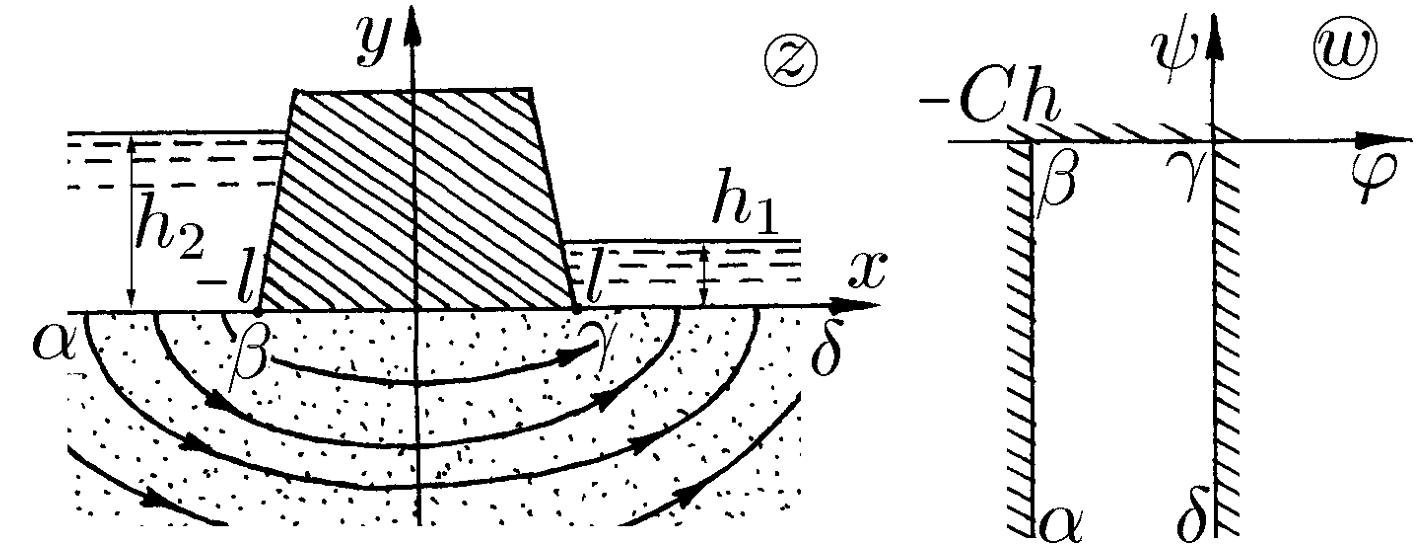
\includegraphics[width=.85\linewidth]{tex_результат/5/figures/figure-15.png}
\caption{}\label{q5:fig-15}
\end{figure}
В этой задаче область течения в плоскости комплексного потенциала $w$ полностью определена и является полубесконечной полосой: на непроницаемом основании плотины $\beta\gamma$ постоянна функция тока $\psi$, которую можно положить равной нулю, а на
дне каждого из водоемов потенциалы скорости фильтрации $\varphi$ принимают постоянные значения. Если значение $\varphi$ на дне $\gamma\delta$ в нижнем бьефе принять равным нулю (добавление константы к $\varphi$ не меняет скорости фильтрации), то на дне $\alpha\beta$ в верхнем бьефе $\varphi=-C(h_2-h_1)=-Ch$, $h=h_2-h_1$.
\source{47--48}
\end{textquote}

% Цитата 8; печатные страницы: 48
\begin{textquote}
Если теперь нам удастся построить (какое-нибудь) конформное отображение нижней полуплоскости в физической плоскости $z$ на полуполосу в плоскости $w$, переводящее точки $\beta$, $\gamma$ и бесконечно удаленную точку $\alpha=\delta$ на плоскости $z$ в их соответствующие образы на плоскости $w$, то такое отображение и будет искомым, т.к. в комплексном анализе доказывается теорема о существовании и единственности конформного отображения области на область, переводящего любые три заданные граничные точки в любые три заданные граничные точки с сохранением порядка их обхода [9].

Несложно проверить, что требуемое отображение имеет вид
\begin{equation}
z=l\cos\left(\frac{\pi}{Ch}w(z)\right).
\tag{8.2}\label{q5:eq-8-2}
\end{equation}
\source{48}
\end{textquote}

% Цитата 9; печатные страницы: 52
\begin{textquote}
Аналогичным образом методы теории аналитических функций применяются при рассмотрении плоскопараллельных горизонтальных течений в плоскости тонкого пласта. В этом случае координатная плоскость $Oxy$ располагается горизонтально, течение описывается уравнениями
\[
\triangle\varphi(x,y)=0,\quad\varphi=-CH(x,y),\quad C=\mathrm{const},\quad\boldsymbol{u}=\grad\varphi,
\]
где напор $H(x,y)=p(x,y,z)/(\rho g)+z$, в силу закона Дарси и предположения о плоскопараллельности течения, не меняется поперек пласта (при этом внутрипластовое давление вдоль любой вертикальной прямой $x=\mathrm{const}$, $y=\mathrm{const}$ распределено по гидростатическому закону).

Простейшие течения, встречающиеся на практике, --- поступательное течение в пласте со скоростью фильтрации $\boldsymbol{U}=(U_x;U_y)$ и течение вокруг работающей совершенной скважины, которое рассматривалось в конце § 7, описываются соответственно комплексными потенциалами $w(z)=\overline{U}z$ и $w(z)=Q/(2\pi)\ln z$, где $U=U_x+iU_y$, а черта над числом обозначает комплексное сопряжение. В силу линейности уравнений можно рассматривать линейные комбинации этих и других решений, что позволяет изучать, например, задачи о гидродинамическом взаимодействии группы скважин.
\source{52}
\end{textquote}

\clearpage\subsection*{Отдельный фрагмент конспекта: труба-источник}
\begin{textquote}
% Источник: porous-lecture-notes.pdf; печатная страница: неизвестна; страница файла: 14; видимый рукописный номер разворота: 14
2. На $z$ форма области течения неизвестна.

Интенсивность источника $2Q$.

\begin{center}
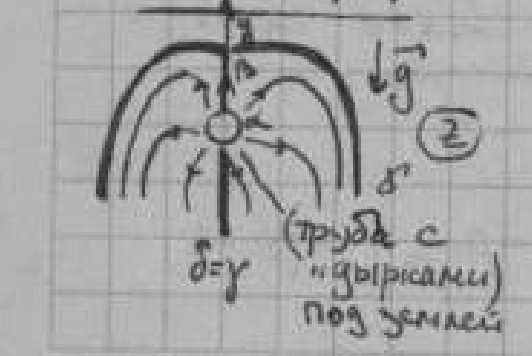
\includegraphics[width=.38\linewidth]{tex_результат/5/figures/notes-physical-domain.png}
\hspace{.04\linewidth}
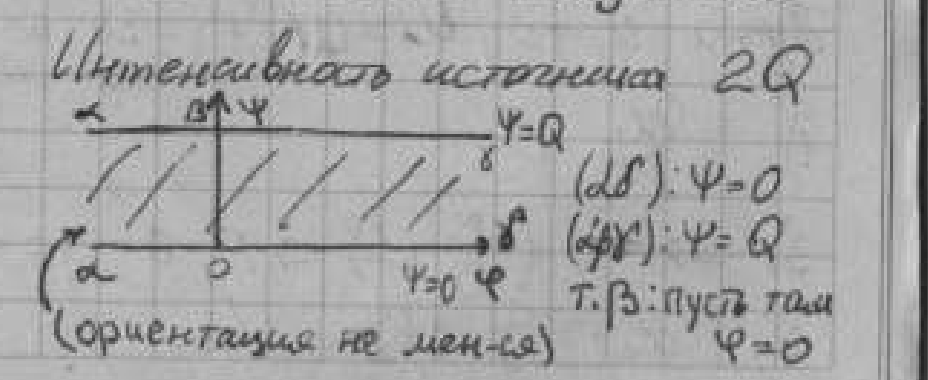
\includegraphics[width=.54\linewidth]{tex_результат/5/figures/notes-potential-domain.png}
\end{center}
Труба с «дырками» под землей.

\[
(\alpha\delta):\ \psi=0,\qquad(\beta\gamma):\ \psi=Q.
\]
Т. $\beta$: пусть там $\varphi=0$.

(ориентация не мен-ся)

% Источник: porous-lecture-notes.pdf; печатная страница: неизвестна; страница файла: 15; видимый рукописный номер разворота: 15
\begin{center}
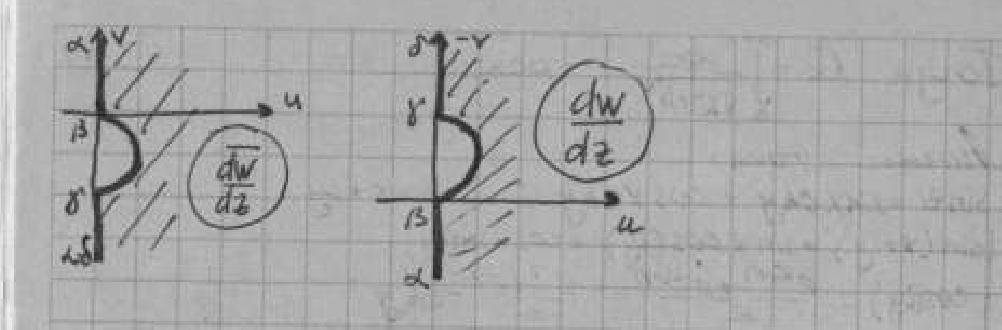
\includegraphics[width=.85\linewidth]{tex_результат/5/figures/notes-hodographs.png}
\end{center}
% На странице файла 15 включены только два рисунка-образа области течения, продолжающие постановку задачи на странице 14. Далее начинается «Гидравлическая теория ф-ции», не входящая в выбранный фрагмент.

\par\nobreak\smallskip{\small Рукописный конспект лекций, \texttt{porous-lecture-notes.pdf}, страницы файла 14--15, видимые рукописные номера разворотов 14 и 15. Автор, год, глава и параграф не указаны. Печатная нумерация не установлена.}
\end{textquote}
\endgroup

\clearpage
\setcounter{questionnumber}{6}
\setcounter{equation}{0}
\setcounter{footnote}{0}
\phantomsection
\section*{Вопрос 6. Безнапорная фильтрация}
\addcontentsline{toc}{section}{Вопрос 6. Безнапорная фильтрация}
\textbf{Формулировка вопроса.} Гидравлическая теория безнапорной фильтрации. Уравнение Буссинеска. Формула Дюпюи для безнапорной фильтрации.

\medskip
\textbf{Где найти.} Леонтьев, 2017; гл. II, § 9, с. 54--58.

\subsection*{Что рассказать}
\begin{enumerate}
\item Условия гидравлического приближения для пологой свободной поверхности; неизвестная высота насыщенного слоя.
\item Гидростатическое распределение давления и закон Дарси в принятом приближении.
\item Уравнение Буссинеска из баланса массы; роль квадрата высоты слоя.
\item Стационарные решения и формулы Дюпюи для безнапорного течения; оговорка о точном расходе через прямоугольную перемычку.
\end{enumerate}
\subsection*{Определения, утверждения, формулы и выводы}
% Исходный ответ: tex_результат/6/6.tex
\begingroup

\begin{quote}\sloppy
Строгое математическое описание безнапорных течений\footnote{Как уже говорилось на стр. 43, \textit{безнапорными} называются течения со свободной поверхностью.}, часто встречающихся в гидрологической практике, достаточно сложно из-за неизвестности формы поверхности депрессии. Для приближенного описания течений со свободной границей французским гидравликом и экономистом Жюлем Дюпюи [19] были предложены упрощающие предположения, которые выполняются для течений с \textit{пологой} поверхностью депрессии.


Рассмотрим (для простоты плоское) нестационарное безнапорное течение несжимаемой жидкости в пористом слое, ограниченном снизу горизонтальной непроницаемой поверхностью (рис.~19). Движение жидкости описывается уравнением неразрывности и законом Дарси, которые в показанной на рисунке системе координат имеют вид\footnote{Для сокращения записи мы будем иногда обозначать частные или обыкновенные производные штрихом, указывая переменную, по которой производится дифференцирование, с помощью нижнего индекса, например: $\frac{\partial p}{\partial x}=p'_x$.}
\begin{equation}\begin{gathered}
\frac{\partial u_x}{\partial x}+\frac{\partial u_z}{\partial z}=0,\qquad u_x=-C\frac{\partial}{\partial x}\left(\frac{p}{\rho g}+z\right)=-C\frac{p'_x}{\rho g},\\
u_z=-C\frac{\partial}{\partial z}\left(\frac{p}{\rho g}+z\right)=-C\left(\frac{p'_z}{\rho g}+1\right).
\end{gathered}\tag{9.1}\label{q6:eq-9-1}\end{equation}
Основное предположение гидравлической теории заключается в том, что при малых углах наклона свободной поверхности к горизонту ($h'_x\ll1$) в любом вертикальном сечении пласта $x=\mathrm{const}$ давление в фильтрующейся жидкости распределено по гидростатическому закону (что эквивалентно постоянству напора по сечению). Если эта гипотеза выполняется, то из закона Дарси следует,
что скорость фильтрации в любой точке направлена горизонтально (ее вертикальная компонента равна нулю), а ее величина определяется только формой свободной поверхности и не зависит от высоты:
\[u_x(x,t)=-Ch'_x,\qquad u_z=0.\]
\par\nobreak\smallskip{\small Н. Е. Леонтьев. \textit{Основы теории фильтрации}. 2-е изд., 2017. Глава II, § 9, с. 54--55.}\par
\end{quote}

\begin{quote}\sloppy
С использованием предположений гидравлической теории легко получить уравнение для высоты свободной поверхности $h(x,t)$, записав закон
сохранения массы для части пористой среды между двумя произвольными сечениями $x_1=\mathrm{const}$ и $x_2=\mathrm{const}$ (рис.~19):
\[\begin{aligned}
\frac{d}{dt}\int_{x_1}^{x_2}\rho mh\,dx&=\left.(\rho h\cdot Ch'_x)\right|_{x_1}^{x_2}=\left.\rho C\left(\frac{h^2}{2}\right)'_x\right|_{x_1}^{x_2}\\
&=C\rho\int_{x_1}^{x_2}\left(\frac{h^2}{2}\right)''_{xx}\,dx,
\end{aligned}\]
откуда получается нелинейное \textit{уравнение Буссинеска} (J. Boussinesq, 1904)
\begin{equation}\frac{\partial h}{\partial t}=\frac{C}{2m}\frac{\partial^2(h^2)}{\partial x^2}.\tag{9.3}\label{q6:eq-9-3}\end{equation}
В общем случае зависимости высоты свободной поверхности от \textit{двух} пространственных координат в горизонтальной плоскости уравнение для $h=h(x,y,t)$ выглядит аналогично:
\[\frac{\partial h}{\partial t}=\frac{C}{2m}\triangle(h^2).\]
В частном случае стационарных течений форма поверхности депрессии находится из уравнения Лапласа
\[\triangle(h^2)=0.\]
\par\nobreak\smallskip{\small Н. Е. Леонтьев. \textit{Основы теории фильтрации}. 2-е изд., 2017. Глава II, § 9, с. 55--56.}\par
\end{quote}

\begin{quote}\sloppy
В случае стационарного плоскопараллельного течения уравнение Буссинеска дает для формы свободной поверхности зависимость
\begin{equation}h^2(x)=Ax+B,\qquad A,B=\mathrm{const}\tag{9.4}\label{q6:eq-9-4}\end{equation}

(для течения слева направо, показанного на рис. 19, $A<0$), для которой постоянный объемный расход жидкости (на единицу длины в поперечном направлении)
\[Q=-Ch'(x)\cdot h(x)=-C(h^2(x)/2)'_x=-CA/2.\]
Записав (9.4) для двух сечений $x_1$ и $x_2$, несложно получить выражение расхода через высоты свободной поверхности в этих точках:
\begin{equation}Q=\frac{C}{2}\frac{h^2(x_1)-h^2(x_2)}{x_2-x_1}.\tag{9.5}\label{q6:eq-9-5}\end{equation}
Аналогичным образом для стационарного осесимметричного безнапорного течения получим решение
\[h^2(r)=A\ln\left(\frac{r}{r_0}\right),\quad A,r_0=\mathrm{const}\]
с расходом
\[Q=-Ch'(r)\cdot2\pi rh(r)=-2\pi rC(h^2(r)/2)'_r=-\pi CA\]
(для притока к скважине, показанного на рис.~20, $A>0$ и расход $Q$ отрицательный). Аналогично плоскому случаю, для расхода можно записать выражение
\begin{equation}Q=-\pi C\frac{h^2(r_2)-h^2(r_1)}{\ln(r_2/r_1)}.\tag{9.6}\label{q6:eq-9-6}\end{equation}
Соотношения (9.5) и (9.6) называются \textit{формулами Дюпюи} для пологой безнапорной фильтрации\setcounter{footnote}{0}\footnote{Сравните с формулой Дюпюи (7.5) на стр. 42.}.
\par\nobreak\smallskip{\small Н. Е. Леонтьев. \textit{Основы теории фильтрации}. 2-е изд., 2017. Глава II, § 9, с. 56--57.}\par
\end{quote}

\begin{quote}\sloppy
Формулы Дюпюи являются приближенными, т.к. при их выводе использовалась приближенная теория. Однако, что любопытно, в случае стационарной фильтрации через прямоугольную перемычку (рис.~21) расход, определяемый по гидравлической теории, совпадает с точным значением, причем при любых (даже немалых) наклонах поверхности депрессии.

\par\nobreak\smallskip{\small Н. Е. Леонтьев. \textit{Основы теории фильтрации}. 2-е изд., 2017. Глава II, § 9, с. 57.}\par
\end{quote}
\endgroup

\clearpage
\setcounter{questionnumber}{7}
\setcounter{equation}{0}
\setcounter{footnote}{0}
\phantomsection
\section*{Вопрос 7. Изотермическая фильтрация газа}
\addcontentsline{toc}{section}{Вопрос 7. Изотермическая фильтрация газа}
\textbf{Формулировка вопроса.} Изотермическая фильтрация газа в недеформируемой пористой среде. Уравнение для давления (уравнение Лейбензона). Аналогия с пологими безнапорными движениями несжимаемой жидкости в пористой среде.

\medskip
\textbf{Где найти.} Леонтьев, 2017; гл. III, § 11, с. 66--69.

\subsection*{Что рассказать}
\begin{enumerate}
\item Изотермичность газа и недеформируемость скелета; какие параметры среды считаются заданными.
\item Уравнения неразрывности и Дарси, уравнение состояния газа и функция Лейбензона.
\item Вывод уравнения для давления; частный случай уравнения Менделеева--Клапейрона.
\item Аналогия полученного уравнения с уравнением Буссинеска для пологих безнапорных течений.
\end{enumerate}
\subsection*{Определения, утверждения, формулы и выводы}
% Исходный ответ: tex_результат/7/7.tex
\begingroup

\begin{quote}\sloppy
При фильтрации газа в промысловых условиях становятся существенными эффекты, связанные с сжимаемостью флюида. В первом приближении можно пренебречь сжимаемостью пористого скелета по сравнению с сжимаемостью газа\footnote{Обычно упругие модули материала скелета (например, модуль Юнга $E$) на много порядков больше давления газа, поэтому относительное изменение удельного объема газа $\delta V/V\sim\delta p/p$ много больше относительных деформаций материала скелета $\varepsilon_{ij}\sim\delta p/E$, вызванных изменениями давления газа.}, считая пористость и проницаемость известными функциями только от пространственных координат:
\[m=m(x,y,z),\qquad k=k(x,y,z),\]
а движение газа (в отсутствие дополнительных источников тепловой энергии) считать \textit{изотермическим}:
\[T(x,y,z,t)=T_0=\mathrm{const}.\]
В этом случае замкнутая система уравнений состоит из уравнения неразрывности и закона Дарси\footnote{Действием массовых сил при фильтрации газа можно пренебречь.}
\[m\frac{\partial\rho}{\partial t}+\Div(\rho\boldsymbol{u})=0,\qquad\boldsymbol{u}=-\frac{k}{\mu}\grad p,\]
к которым добавляются известные уравнения состояния для газа:
\[\rho=\rho(p,T_0)=\rho(p),\qquad\mu=\mu(p,T_0)=\mu(p).\]
\par\nobreak\smallskip{\small Н. Е. Леонтьев. \textit{Основы теории фильтрации}. 2-е изд., 2017. Глава III, § 11, с. 66.}\par
\end{quote}

\begin{quote}\sloppy
Из этих уравнений можно получить одно уравнение относительно давления. Действительно, подставляя закон Дарси в уравнение неразрывности и для простоты полагая пористость и проницаемость постоянными величинами, получим уравнение
\[m\frac{d\rho(p)}{dp}\frac{\partial p}{\partial t}=k\Div\left(\frac{\rho(p)}{\mu(p)}\grad p\right),\]
которое после введения \textit{функции Лейбензона}\setcounter{footnote}{0}\footnote{Функция Лейбензона монотонно возрастает, и, следовательно, может быть обращена: $p=p(\mathscr{P})$.}
\[\mathscr{P}(p)=k\int_0^p\frac{\rho(p_1)}{\mu(p_1)}\,dp_1\]
приобретает вид нелинейного уравнения относительно $\mathscr{P}$:
\[\frac{\partial\mathscr{P}}{\partial t}=\varkappa(\mathscr{P})\cdot\triangle\mathscr{P},\quad\varkappa(\mathscr{P})=\varkappa(\mathscr{P}(p))=\frac{k\rho(p)}{m\mu(p)}\frac{dp(\rho)}{d\rho}.\]
Обратим внимание, что функции $\mathscr{P}(p)$ и $\varkappa(p)$ зависят только от свойств газа и являются \textit{известными} до решения задачи.

В частном случае газа с уравнением состояния Менделеева--Клапейрона и постоянной вязкостью $\mu=\mathrm{const}$\footnote{Вязкость газа из невзаимодействующих частиц, как это устанавливается в молекулярно-кинетической теории, не зависит от давления и увеличивается с ростом температуры по закону $\mu\sim\sqrt T$. Вязкость реальных газов при $T=\mathrm{const}$ как правило возрастает с повышением давления.} эти формулы дают
\[\begin{gathered}
p=\frac{p_0}{\rho_0}\rho,\quad\mathscr{P}(p)=\frac{k\rho_0}{2\mu p_0}p^2,\quad\varkappa(\mathscr{P}(p))=\frac{k}{m\mu}p,\\
\frac{\partial(p^2)}{\partial t}=\frac{k}{m\mu}p\triangle(p^2),
\end{gathered}\]
откуда получается \textit{уравнение Лейбензона}\footnote{Уравнение (11.1) было получено в начале 1920-х гг. академиком Л.С.Лейбензоном и несколько позже американским гидромехаником М.Маскетом (M.Muskat).}
\begin{equation}\frac{\partial p}{\partial t}=\frac{k}{2m\mu}\triangle(p^2),\tag{11.1}\label{q7:eq-11-1}\end{equation}
которое совпадает с уравнением Буссинеска (9.3) для формы пологой поверхности депрессии при безнапорной фильтрации несжимаемой жидкости.
\par\nobreak\smallskip{\small Н. Е. Леонтьев. \textit{Основы теории фильтрации}. 2-е изд., 2017. Глава III, § 11, с. 66--67.}\par
\end{quote}
\endgroup

\clearpage
\setcounter{questionnumber}{8}
\setcounter{equation}{0}
\setcounter{footnote}{0}
\phantomsection
\section*{Вопрос 8. Упругий режим и пьезопроводность}
\addcontentsline{toc}{section}{Вопрос 8. Упругий режим и пьезопроводность}
\textbf{Формулировка вопроса.} Упругий режим фильтрации. Уравнение пьезопроводности. Постановка задачи о распространении плоской волны повышения давления в полубесконечном пласте. Оценка характерного времени распространения возмущения давления.

\medskip
\textbf{Где найти.} Леонтьев, 2017; гл. III, § 12, с. 70--77.

\subsection*{Что рассказать}
\begin{enumerate}
\item Упругий режим: малые изменения плотности жидкости и свойств пористого скелета; линейные соотношения состояния.
\item Вывод уравнения пьезопроводности, отбрасывание нелинейного члена и коэффициент пьезопроводности.
\item Плоская волна повышения давления: полубесконечный пласт, начальное условие и условия на границе и бесконечности.
\item Автомодельная переменная, решение через функцию ошибок, скорость фильтрации и оценка времени $\tau\sim L^2/\varkappa$.
\end{enumerate}
\subsection*{Определения, утверждения, формулы и выводы}
% Исходный ответ: tex_результат/8/8.tex
\begingroup

\begin{quote}\sloppy
В отличие от газов, которые могут в разы менять свой объем, капельные жидкости (вода, нефть) являются \textit{слабосжимаемыми} веществами, у которых в промысловых условиях относительное изменение объема составляет доли процента. Поэтому, во-первых, при изучении эффектов сжимаемости на фильтрацию жидкостей нужно одновременно учитывать и сжимаемость пористого скелета и, во-вторых, учет этих изменений можно проводить в линейном приближении.

В соответствии с этим к системе, состоящей из уравнения неразрывности и закона Дарси:
\[
(m\rho)'_t+\Div(\rho\boldsymbol u)=0,\qquad \boldsymbol u=-\frac{k}{\mu}\grad p,
\]
добавляются \textit{линейные} соотношения, определяющие изотермические зависимости плотности $\rho$, пористости $m$, проницаемости $k$ и вязкости $\mu$ от возмущения давления жидкости в порах по сравнению с некоторым начальным состоянием $p_0$\footnote{Тем самым мы предполагаем деформации жидкости и пористого скелета \textit{обратимыми} (упругими), в связи с чем о процессах, при которых эта теория справедлива, говорят как об \textit{упругом режиме фильтрации}.}:
\begin{equation}\begin{aligned}
\rho(p)&=\rho_0\cdot\left(1+\frac{p-p_0}{K_\rho}\right),&m(p)&=m_0\cdot\left(1+\frac{p-p_0}{K_m}\right),\\
k(p)&=k_0\cdot\left(1+\frac{p-p_0}{K_k}\right),&\mu(p)&=\mu_0\cdot\left(1+\frac{p-p_0}{K_\mu}\right),
\end{aligned}\tag{12.1}\label{q8:eq-12-1}\end{equation}
где величины $\rho_0,m_0,k_0,\mu_0$ относятся к невозмущенному состоянию, а константы $K_\rho,K_m,K_k,K_\mu$ являются упругими модулями\footnote{Например, при $10^\circ$C для воды $K_\rho\approx2\cdot10^4$ атм, $K_\mu\approx-2\cdot10^4$ атм; отрицательное значение $K_\mu$ соответствует падению вязкости воды при не очень большом повышении давления.}, которые характеризуют изменение свойств пористой среды и жидкости при всестороннем сжатии и по порядку величины много больше характерных возмущений давления: $(p-p_0)/K\ll1$.

\setcounter{footnote}{0}
\par\nobreak\smallskip{\small Н. Е. Леонтьев. \textit{Основы теории фильтрации}. 2-е изд., 2017. Глава III, § 12, с. 70.}\par
\end{quote}

\begin{quote}\sloppy
Как и в случае фильтрации газа (§ 11), мы подставим закон Дарси в уравнение неразрывности:
\[
\frac{\partial(m(p)\rho(p))}{\partial t}=\Div\left(\frac{\rho(p)k(p)}{\mu(p)}\grad p\right),
\]
что после преобразований дает
\[
\rho m\left(\frac{m'_p}{m}+\frac{\rho'_p}{\rho}\right)p'_t=\frac{\rho k}{\mu}\left\{\left(\frac{\rho'_p}{\rho}+\frac{k'_p}{k}+\frac{(1/\mu)'_p}{1/\mu}\right)|\grad p|^2+\Delta p\right\},
\]
и, поскольку мы хотим получить уравнения для \textit{малых возмущений}, упростим коэффициенты при производных от давления: вместо значений $k,\mu,\rho$ и $m$ возьмем их невозмущенные значения $k_0,\mu_0,\rho_0$ и $m_0$, а при вычислении производных воспользуемся линейными уравнениями состояния (12.1), например:
\[
\frac{\rho'_p}{\rho}\approx\frac{1}{K_\rho},\qquad \frac{(1/\mu)'_p}{1/\mu}\approx-\frac{1}{K_\mu}.
\]
В результате получится уравнение с постоянными коэффициентами, в котором дополнительно можно отбросить нелинейное слагаемое\footnote{Зачеркнутый член имеет порядок $(p-p_0)^2/(KL^2)$, где $L$ --- характерный размер задачи, а оператор Лапласа порядка $(p-p_0)/L^2$, так что отношение этих членов порядка $(p-p_0)/K\ll1$.}:
\[
\rho_0m_0\left(\frac{1}{K_m}+\frac{1}{K_\rho}\right)p'_t=\frac{\rho_0k_0}{\mu_0}\left\{\cancel{\left(\frac{1}{K_\rho}+\frac{1}{K_k}-\frac{1}{K_\mu}\right)|\grad p|^2}+\Delta p\right\},
\]
что в итоге дает \textit{уравнение пьезопроводности}\footnote{Название (от греч. $\pi\iota\varepsilon\zeta\omega$ --- «давлю») дано по аналогии с названием уравнения теплопроводности, совпадающего по форме с (12.2).}, полученное рядом исследователей в 1930--40-х гг. [11,17]:
\begin{equation}
p'_t=\varkappa\Delta p,\qquad \varkappa=\frac{k_0}{m_0\mu_0}\left(\frac{1}{K_\rho}+\frac{1}{K_m}\right)^{-1}=\mathrm{const},\tag{12.2}\label{q8:eq-12-2}
\end{equation}
где $\varkappa$ --- \textit{коэффициент пьезопроводности}. Граничные условия для уравнения (12.2) ставятся аналогично условиям при изотермической фильтрации газа (стр. 67).

\setcounter{footnote}{0}
Коэффициент пьезопроводности одновременно учитывает сжимаемость жидкости и пористого скелета. Отметим, что в промысловых условиях встречаются ситуации, когда фильтрующаяся жидкость содержит пузырьки газа (например, газ, растворенный в жидкости, может выделяться при понижении давления). Это приводит к увеличению средней сжимаемости флюида и, как следствие, к резкому снижению эффективного коэффициента пьезопроводности $\varkappa$.
\par\nobreak\smallskip{\small Н. Е. Леонтьев. \textit{Основы теории фильтрации}. 2-е изд., 2017. Глава III, § 12, с. 71--72.}\par
\end{quote}

\begin{quote}\sloppy
Рассмотрим одномерную задачу движении плоской волны давления в полубесконечном пористом пласте. Предположим, что начальное давление флюида в пласте постоянно, а в нулевой момент времени давление на границе пласта \textit{скачком} повышается на постоянную величину $\delta p$ и далее все время поддерживается на этом уровне. Считая для простоты начальное давление нулевым: $p_0=0$\footnote{В уравнение пьезопроводности входят только производные от давления.} и направляя ось $Ox$ вдоль пласта, получим задачу
\begin{equation}
p'_t=\varkappa p''_{xx},\quad p(x,0)=0,\quad p(0,t)=\delta p,\quad \lim_{x\to\infty}p(x,t)=0\tag{12.3}\label{q8:eq-12-3}
\end{equation}
(начало координат выбрано на границе пласта). Решение задачи автомодельно и, в соответствии с $\pi$-теоремой, имеет вид
\[
p=p(x,t,\varkappa,\delta p)=\delta p\cdot f(\xi),\qquad \xi=\frac{x}{\sqrt{\varkappa t}},
\]
что сводит (12.3) к краевой задаче для обыкновенного дифференциального уравнения
\[
2f''(\xi)+\xi f'(\xi)=0,\quad f(0)=1,\quad f(\infty)=0,
\]
решение которой выражается через функцию ошибок (рис. 27 \textit{а}):
\[
f(\xi)=1-\operatorname{erf}(\xi/2),\qquad \operatorname{erf}x=\frac{2}{\sqrt\pi}\int_0^x\exp(-\alpha^2)\,d\alpha.
\]
В размерных переменных распределение давления дается выражением
\[
p(x,t)=\delta p\cdot\left(1-\operatorname{erf}\left(\frac{x}{2\sqrt{\varkappa t}}\right)\right);
\]
качественный вид пространственного распределения давления для трех моментов времени $t_1<t_2<t_3$ показан на рис. 27 \textit{б}.


Скорость фильтрации, которая находится с помощью закона Дарси:
\[\begin{aligned}
u_x(x,t)&=-\frac{k(p(x,t))}{\mu(p(x,t))}p'_x(x,t)\approx-\frac{k_0}{\mu_0}p'_x(x,t)=\\
&=\frac{k_0\delta p}{\mu_0}\frac{1}{\sqrt{\pi\varkappa t}}\exp\left(-\frac{x^2}{4\varkappa t}\right),
\end{aligned}\]
в каждой фиксированной внутренней точке пласта с течением времени сначала возрастает от нулевого значения до некоторого максимального, а затем постепенно падает до нуля при $t\to\infty$ (рис. 27 \textit{в}).

С помощью этого решения несложно оценить характерное время $\tau$ переходного процесса в упругом режиме: $\tau\sim L^2/\varkappa$. При характерных параметрах $K\sim10^4$ атм, $k\sim10^{-8}$ см$^2$, $\mu\sim10^{-2}$ г/(см$\cdot$с), $m\sim1$ получим $\varkappa\sim1$ м$^2$/с, и если $L\sim10$ м, то $\tau\sim1$ мин, а при $L\sim10^3$ м $\tau\sim10$ сут.
\par\nobreak\smallskip{\small Н. Е. Леонтьев. \textit{Основы теории фильтрации}. 2-е изд., 2017. Глава III, § 12, с. 72--73.}\par
\end{quote}
\endgroup

\clearpage
\setcounter{questionnumber}{9}
\setcounter{equation}{0}
\setcounter{footnote}{0}
\phantomsection
\section*{Вопрос 9. Поршневое вытеснение и устойчивость фронта}
\addcontentsline{toc}{section}{Вопрос 9. Поршневое вытеснение и устойчивость фронта}
\textbf{Формулировка вопроса.} Вытеснение несмешивающихся жидкостей. Одномерная задача о поршневом вытеснении несмешивающихся жидкостей (модель Лейбензона — Маскета). Устойчивость фронта вытеснения (элементарная теория).

\medskip
\textbf{Где найти.} Басниев, Власов, Кочина, Максимов, \textit{Подземная гидравлика}, 1986; гл. 8, §§ 1, 2, 4, с. 188--193, 196--198.

\subsection*{Что рассказать}
\begin{enumerate}
\item Поршневое вытеснение: несмешиваемость, несжимаемость, полнота вытеснения и условия на границе раздела.
\item Прямолинейная задача при постоянных граничных давлениях: распределения давления, общий поток и давление на фронте.
\item Закон движения фронта из связи скорости фильтрации со скоростью границы; время полного вытеснения.
\item Элементарная теория устойчивости: сравнение скоростей возмущённой и основной фаз, влияние вязкости, плотности и наклона пласта.
\end{enumerate}
\subsection*{Определения, утверждения, формулы и выводы}
% Исходный ответ: tex_результат/9/9.tex
\begingroup

\begin{quote}\sloppy
Согласно условию неразрывности потока массы элементарные расходы обеих несжимаемых жидкостей через элемент границы раздела, включающий точку $M$, должны быть равны между собой. Отсюда следует, что нормальные составляющие скоростей фильтрации обеих жидкостей будут равны, т. е. $w_{1n}=w_{2n}$. Давление в пласте в точке $M$ также должно быть одинаково для обеих жидкостей, так как при малых скоростях (ниже звуковых) разрыва давления в сплошном потоке быть не может.
\par\nobreak\smallskip
{\small К. С. Басниев, А. М. Власов, И. Н. Кочина, В. М. Максимов. \textit{Подземная гидравлика}. 1986. Глава 8, § 1, с. 188.}\par
\end{quote}

\begin{quote}\sloppy
Линии тока не будут преломляться только в двух случаях --- при прямолинейно-параллельном и плоскорадиальном движениях границы раздела, когда $w_{1\tau}=w_{2\tau}=0$. Эти задачи прежде всего и будут рассмотрены в данной главе. При этом жидкости (нефть и вода) считаются несжимаемыми, взаимно нерастворимыми и химически не реагирующими одна с другой и с пористой средой. Вытеснение нефти водой предполагается происходящим полностью --- так называемое поршневое вытеснение. Задачи, в которых учитывается неполнота вытеснения, рассматриваются в гл. 9.
\par\nobreak\smallskip
{\small К. С. Басниев, А. М. Власов, И. Н. Кочина, В. М. Максимов. \textit{Подземная гидравлика}. 1986. Глава 8, § 1, с. 189.}\par
\end{quote}

\begin{quote}\sloppy
При поршневом вытеснении нефти водой в пористой среде плотности нефти и воды будем считать одинаковыми. Это позволит рассматривать плоскость контакта нефти и воды вертикальной. А различие в вязкостях нефти $\mu_\text{н}$ и воды $\mu_\text{в}$ будем учитывать.

В случае прямолинейно-параллельного движения схема вытеснения представлена на рис. 8.2. На контуре питания и на галерее поддерживаются соответственно постоянные давления $p_\text{к}$ и $p_\text{г}$. Начальное положение контура нефтеносности $x_0$ параллельно галерее и контуру питания.

Обозначим через $x_\text{в}$ текущее расстояние до контура нефтеносности в момент времени $t$ после начала вытеснения, через $L_\text{к}$ --- расстояние от контура питания до галереи, через $p_\text{в},p_\text{н}$ --- давление в любой точке водоносной и нефтеносной части пласта соответственно, через $p(t)$ --- давление на границе раздела вода---нефть, отстоящей от контура питания на расстоянии $x_\text{в}$.
\par\nobreak\smallskip
{\small К. С. Басниев, А. М. Власов, И. Н. Кочина, В. М. Максимов. \textit{Подземная гидравлика}. 1986. Глава 8, § 2, с. 189.}\par
\end{quote}

\begin{quote}\sloppy
При этом изобарами являются линии, параллельные галерее, и каждую изобару можно рассматривать как контур питания или как галерею. На основании формул (8.3) и (8.4) распределение давления и скорость фильтрации в водоносной области можно записать в виде
\begin{equation}p_\text{в}=p_\text{к}-\frac{p_\text{к}-p(t)}{x_\text{в}(t)}x,\quad0\le x\le x_\text{в}(t);\tag{8.5}\label{q9:eq-8-5}\end{equation}
\begin{equation}w_\text{в}=\frac{k}{\mu_\text{в}}\frac{p_\text{к}-p(t)}{x_\text{в}(t)}.\tag{8.6}\label{q9:eq-8-6}\end{equation}
Принимая за контур питания изобару, совпадающую с границей раздела жидкостей, распределение давления и скорость фильтрации в нефтеносной области можно записать следующим образом:
\begin{equation}p_\text{н}=p_\text{г}+\frac{p(t)-p_\text{г}}{L_\text{к}-x_\text{в}(t)}(L_\text{к}-x),\quad x_\text{в}(t)\le x\le L_\text{к};\tag{8.7}\label{q9:eq-8-7}\end{equation}
\begin{equation}w_\text{н}=\frac{k}{\mu_\text{н}}\frac{p(t)-p_\text{г}}{L_\text{к}-x_\text{в}(t)}.\tag{8.8}\label{q9:eq-8-8}\end{equation}
Найдем давление $p(t)$ на границе раздела. Вследствие несжимаемости жидкостей и неразрывности потока линии тока будут иметь вид прямых, параллельных оси $Ox$ (на границе раздела преломления не будет), а скорость фильтрации во всех точках пласта будет одинаковой, т. е. $w_\text{в}=w_\text{н}$.

Тогда из уравнений (8.6) и (8.8) получим
\begin{equation}\frac{k(p_\text{к}-p(t))}{\mu_\text{в}x_\text{в}(t)}=\frac{k(p(t)-p_\text{г})}{\mu_\text{н}(L_\text{к}-x_\text{в}(t))},\tag{8.9}\label{q9:eq-8-9}\end{equation}
откуда давление на границе раздела жидкостей будет
\begin{equation}p(t)=\frac{p_\text{к}\mu_\text{н}(L_\text{к}-x_\text{в}(t))+p_\text{г}\mu_\text{в}x_\text{в}(t)}{\mu_\text{в}x_\text{в}(t)+\mu_\text{н}(L_\text{к}-x_\text{в}(t))}.\tag{8.10}\label{q9:eq-8-10}\end{equation}
\par\nobreak\smallskip
{\small К. С. Басниев, А. М. Власов, И. Н. Кочина, В. М. Максимов. \textit{Подземная гидравлика}. 1986. Глава 8, § 2, с. 190.}\par
\end{quote}

\begin{quote}\sloppy
2. Скорость фильтрации. Подставим (8.10) в (8.6) и (8.8):
\begin{equation}w_\text{в}=w_\text{н}=\frac{k(p_\text{к}-p_\text{г})}{\mu_\text{в}x_\text{в}(t)+\mu_\text{н}(L_\text{к}-x_\text{в}(t))}.\tag{8.13}\label{q9:eq-8-13}\end{equation}
\par\nobreak\smallskip
{\small К. С. Басниев, А. М. Власов, И. Н. Кочина, В. М. Максимов. \textit{Подземная гидравлика}. 1986. Глава 8, § 2, с. 190.}\par
\end{quote}

\begin{quote}\sloppy
5. Закон движения границы раздела $x_\text{в}=x_\text{в}(t)$ находим из соотношения скорости фильтрации и средней скорости движения:
\[w=mv=m\frac{dx_\text{в}}{dt},\]
откуда
\begin{equation}dt=\frac{m}{w}dx_\text{в}=\frac{m}{\dfrac{k(p_\text{к}-p_\text{г})}{\mu_\text{в}x_\text{в}(t)+\mu_\text{н}(L_\text{к}-x_\text{в}(t))}}dx_\text{в}.\tag{8.17}\label{q9:eq-8-17}\end{equation}
Проинтегрировав (8.17) в пределах от 0 до $t$ и от $x_0$ до $x_\text{в}$, получим
\begin{equation}t=\frac{m}{k(p_\text{к}-p_\text{г})}\left[\mu_\text{н}L_\text{к}(x_\text{в}-x_0)-\frac12(\mu_\text{н}-\mu_\text{в})(x_\text{в}^2-x_0^2)\right].\tag{8.18}\label{q9:eq-8-18}\end{equation}
Чтобы найти время полного вытеснения нефти, нужно в формуле (8.18) положить $x_\text{в}=L_\text{к}$. Тогда получим
\[T=\frac{m}{2k(p_\text{к}-p_\text{г})}\left[\mu_\text{в}(L_\text{к}^2-x_0^2)+\mu_\text{н}(L_\text{к}-x_0)^2\right].\]
\par\nobreak\smallskip
{\small К. С. Басниев, А. М. Власов, И. Н. Кочина, В. М. Максимов. \textit{Подземная гидравлика}. 1986. Глава 8, § 2, с. 191.}\par
\end{quote}

\begin{quote}\sloppy
Пусть нефтяная залежь в наклонном пласте (рис. 8.6) имеет горизонтальное начальное положение водонефтяного контакта $A_0B_0$.

При отборе нефти граница раздела вода---нефть будет перемещаться, занимая последовательно положения $A_1B_1$, $A_2B_2$ и т. д. Рассмотрим вопрос об устойчивости движения границы раздела. Скорости фильтрации каждой жидкости согласно закону Дарси определяются при учете силы тяжести по формулам
\begin{equation}\begin{aligned}
w_\text{в}&=-\frac{k_1}{\mu_\text{в}}\left(\frac{\partial p}{\partial s}+\rho_\text{в}g\frac{\partial z}{\partial s}\right);&w_\text{н}&=-\frac{k_2}{\mu_\text{н}}\left(\frac{\partial p}{\partial s}+\rho_\text{н}g\frac{\partial z}{\partial s}\right).
\end{aligned}\tag{8.39}\label{q9:eq-8-39}\end{equation}
Вследствие неизбежных возмущений на границе раздела частицы воды попадают в область, занятую нефтью, при этом их дальнейшее движение может либо ускоряться, либо замедляться. В первом случае, при ускорении движения частиц воды, движение границы раздела будет неустойчивым; во втором, при замедлении движения частиц воды, --- устойчивым.


Условия устойчивости движения границы раздела можно установить из следующих элементарных соображений. Обозначим через $(w_\text{в})_\text{н}$ скорость фильтрации частиц воды, попавших в поток нефти с градиентом давления $(\partial p/\partial s)_\text{н}$; через $(k_1)_2$ --- проницаемость пласта для воды в зоне движения нефти.

Тогда из первого соотношения (8.39) имеем
\begin{equation}(w_\text{в})_\text{н}=-\frac{(k_1)_2}{\mu_\text{в}}\left[\left(\frac{\partial p}{\partial s}\right)_\text{н}+\rho_\text{в}g\frac{\partial z}{\partial s}\right].\tag{8.40}\label{q9:eq-8-40}\end{equation}
Скорость фильтрации основных частиц нефти, соприкасающихся с проникшими туда частицами воды, согласно второму уравнению (8.39) будет
\begin{equation}w_\text{н}=-\frac{k_2}{\mu_\text{н}}\left[\left(\frac{\partial p}{\partial s}\right)_\text{н}+\rho_\text{н}g\frac{\partial z}{\partial s}\right].\tag{8.41}\label{q9:eq-8-41}\end{equation}
Из уравнений (8.40) и (8.41) получаем связь между скоростями фильтрации $(w_\text{в})_\text{н}$ и $w_\text{н}$:
\[
\frac{\mu_\text{в}}{(k_1)_2}(w_\text{в})_\text{н}+\rho_\text{в}g\frac{\partial z}{\partial s}=\frac{\mu_\text{н}}{k_2}w_\text{н}+\rho_\text{н}g\frac{\partial z}{\partial s}=-\left(\frac{\partial p}{\partial s}\right)_\text{н},
\]
откуда
\[
(w_\text{в})_\text{н}=\frac{\mu_\text{н}}{\mu_\text{в}}\frac{(k_1)_2}{k_2}w_\text{н}-\frac{(k_1)_2}{\mu_\text{в}}(\rho_\text{в}-\rho_\text{н})g\frac{\partial z}{\partial s}.
\]
Об устойчивости движения границы раздела можно судить по разности скоростей фильтрации:
\begin{equation}\begin{aligned}
\Delta w&=(w_\text{в})_\text{н}-w_\text{н}=\left[\frac{\mu_\text{н}}{\mu_\text{в}}\frac{(k_1)_2}{k_2}-1\right]w_\text{н}-\\
&\quad-\frac{(k_1)_2}{\mu_\text{в}}(\rho_\text{в}-\rho_\text{н})g\frac{\vert\partial z}{\partial s}.
\end{aligned}\tag{8.42}\label{q9:eq-8-42}\end{equation}
При $\Delta w\le0$ движение границы раздела жидкостей будет устойчивым, при $\Delta w\ge0$ движение неустойчиво.

Если угол наклона пласта к горизонту обозначить через $\alpha$, то, очевидно, $\partial z/\partial s=\sin\alpha$.

Тогда условие устойчивости границы раздела (8.42) можно представить в виде
\[
\Delta w=\left[\frac{\mu_\text{н}}{\mu_\text{в}}\frac{(k_1)_2}{k_2}-1\right]w_\text{н}-\frac{(k_1)_2}{\mu_\text{в}}(\rho_\text{в}-\rho_\text{н})g\sin\alpha.
\]
Обычно $(k_1)_2$ меньше $k_2$. Считая в первом приближении, что $(k_1)_2=k_2$, преобразуем это соотношение к виду
\begin{equation}\Delta w=\left(\frac{\mu_\text{н}}{\mu_\text{в}}-1\right)w_\text{н}-\frac{k_2}{\mu_\text{в}}(\rho_\text{в}-\rho_\text{н})g\sin\alpha.\tag{8.43}\label{q9:eq-8-43}\end{equation}
Так как при устойчивом движении границы раздела $\Delta w\le0$, то из (8.43) найдем, что при устойчивом движении границы раздела жидкостей скорость фильтрации нефти $w_\text{н}$ на границе раздела должна быть
\[
w_\text{н}\le\frac{k_2}{\mu_\text{н}-\mu_\text{в}}(\rho_\text{в}-\rho_\text{н})g\sin\alpha.
\]
Более строгое исследование рассмотренной задачи проводится методами теории возмущений и гидродинамической устойчивости.
\par\nobreak\smallskip
{\small К. С. Басниев, А. М. Власов, И. Н. Кочина, В. М. Максимов. \textit{Подземная гидравлика}. 1986. Глава 8, § 4, с. 197--198.}\par
\end{quote}

\noindent В формуле (8.42) перед $\partial z$ на скане виден дополнительный вертикальный штрих. Это место требует сверки с более чётким изображением оригинала; штрих сохранён.
\endgroup

\clearpage
\setcounter{questionnumber}{10}
\setcounter{equation}{0}
\setcounter{footnote}{0}
\phantomsection
\section*{Вопрос 10. Многофазная фильтрация и капиллярность}
\addcontentsline{toc}{section}{Вопрос 10. Многофазная фильтрация и капиллярность}
\textbf{Формулировка вопроса.} Описание многофазной фильтрации. Обобщенный закон Дарси, относительная фазовая проницаемость. Учет капиллярной разности давлений между фазами, функция Леверетта.

\medskip
\textbf{Где найти.} Басниев и др., 1986; гл. 1, § 5, с. 19--22; гл. 9, §§ 2--3, с. 199--204.

\subsection*{Что рассказать}
\begin{enumerate}
\item Фазы, насыщенности и скорости фильтрации; число независимых насыщенностей.
\item Фазовая и относительная проницаемости; обобщённый закон Дарси и условия совместного движения фаз.
\item Разность давлений между фазами, капиллярное давление и безразмерная функция Леверетта.
\item Уравнения сохранения массы каждой фазы и замыкающие соотношения; предположения о равновесии, гистерезисе и фазовых переходах.
\end{enumerate}
\subsection*{Определения, утверждения, формулы и выводы}
% Исходный ответ: tex_результат/10/10.tex
\begingroup

\begin{quote}\sloppy
Углеводородные системы могут быть гомо- и гетерогенными. В гомогенной системе все ее части имеют одинаковые физические и химические свойства. Составляющие гомогенной системы (называемые компонентами) «размазаны» по всему пространству и взаимодействуют на молекулярном уровне. Для гетерогенной системы физические и химические свойства в разных точках различны. Гетерогенные системы состоят из фаз. Фаза --- это часть системы, которая является гомогенной и отделена от других фаз отчетливыми границами. Смесь воды, нефти и газа в пласте --- типичный пример гетерогенной среды.

Главными характеристиками движения многофазной системы являются насыщенность и скорость фильтрации каждой фазы.

Насыщенностью $\sigma_i$ порового пространства $i$-й фазой называется доля объема пор $\Delta V_i$, занятая этой фазой в элементарном объеме:
\begin{equation}\sigma_i=\Delta V_i/\Delta V_\text{п},\quad i=1,2,\ldots,n.\tag{9.1}\label{q10:eq-9-1}\end{equation}
Очевидно, что
\begin{equation}\sum_{i=1}^n\sigma_i=1.\tag{9.2}\label{q10:eq-9-2}\end{equation}
Таким образом, в $n$-фазной системе имеется $(n-1)$ независимая насыщенность. В частности, при исследовании фильтрации смеси двух фаз используется лишь одна из насыщенностей, которая обозначается в дальнейшем $\sigma$ (обычно это насыщенность вытесняющей фазы).

Движение каждой из фаз характеризуется вектором скорости фильтрации $\vec w_i$ данной фазы, который (по аналогии со скоростью фильтрации однородной жидкости) определяется как вектор, проекция которого на некоторое направление $l$ равна отношению объемного расхода $Q_i$ данной фазы к площадке $\Omega_l$, перпендикулярной к указанному направлению:
\begin{equation}(\vec w_i)_l=Q_i/\Omega_l,\quad i=1,2,\ldots,n.\tag{9.3}\label{q10:eq-9-3}\end{equation}
Площадка $\Omega_l$ пересекает как твердую, так и подвижные фазы.
\par\nobreak\smallskip{\small К. С. Басниев, А. М. Власов, И. Н. Кочина, В. М. Максимов. \textit{Подземная гидравлика}. Москва: Недра, 1986. Глава 9, § 2, с. 199--200.}\par
\end{quote}

\begin{quote}\sloppy
Экспериментально установлено, что расход каждой фазы растет с увеличением перепада давления и насыщенности данной фазой, а закон фильтрации каждой из фаз по аналогии с законом Дарси можно записать в виде
\begin{equation}w_1=\frac{k_1^*\Delta p_1}{\mu_1L},\qquad w_2=\frac{k_2^*\Delta p_2}{\mu_2L},\tag{1.18}\label{q10:eq-1-18}\end{equation}
где $w_1$ и $w_2$ --- скорости фильтрации фаз; $\mu_1$ и $\mu_2$ --- динамические коэффициенты вязкости жидкостей; $\Delta p_1$ и $\Delta p_2$ --- разности давлений в соответствующих фазах; $k_1^*$ и $k_2^*$ --- фазовые проницаемости. Величины $k_i^*$ ($i=1,2$) являются для $i$-й жидкости проницаемостями в обычном смысле в условиях совместной фильтрации. Эти величины зависят от природы пористой среды (и, прежде всего, от ее абсолютной проницаемости $k$, определяемой по данным о фильтрации однородной жидкости), а также от насыщенности пористой среды каждой фазой. При описании двухфазных течений обычно вместо фазовых проницаемостей $k_i^*$ вводят так называемые
«относительные проницаемости» $k_i$ фаз, определяемые из отношений
\begin{equation}k_1=k_1^*/k,\qquad k_2=k_2^*/k.\tag{1.19}\label{q10:eq-1-19}\end{equation}
В большинстве опытов показано, что для данной структуры пористой среды относительные проницаемости $k_i$ являются в основном функциями насыщенности, а если и наблюдается влияние иных параметров (например, отношения коэффициентов вязкости $\mu_0$ фаз), то им обычно пренебрегают. Тогда с учетом (1.19) закон Дарси (1.18) для каждой из фаз записывается в виде
\begin{equation}w_i=k\frac{k_i(\sigma)\Delta p_i}{\mu_iL},\qquad i=1,2.\tag{1.20}\label{q10:eq-1-20}\end{equation}
\par\nobreak\smallskip{\small К. С. Басниев, А. М. Власов, И. Н. Кочина, В. М. Максимов. \textit{Подземная гидравлика}. Москва: Недра, 1986. Глава 1, § 5, с. 19--20.}\par
\end{quote}

\begin{quote}\sloppy
Типичный вид экспериментальных кривых фазовых проницаемостей $k_i(\sigma)$ приведен на рис. 1.6 (кривая \textit{1} относится к более смачивающей жидкости --- воде, кривая \textit{2} --- к менее смачивающей --- нефти; кривая $1'$ относится к случаю, когда первая фаза является газом и $\sigma$ --- газонасыщенность). Отметим некоторые характерные особенности этих кривых. Для каждой фазы существует предельная насыщенность ($\sigma_*$ и $1-\sigma^*$) такая, что при меньших значениях насыщенности эта фаза неподвижна. Движение первой фазы может происходить только в том случае, если $\sigma>\sigma_*$ (для водонефтяной системы $\sigma_*$ называют насыщенностью связанной водой). Для второй фазы связанная насыщенность равна $1-\sigma^*$ и называется остаточной нефтенасыщенностью. Таким образом, совместное течение двух фаз имеет место лишь в следующем интервале изменения насыщенности жидкостью 1:
\[\sigma_*\le\sigma\le\sigma^*.\]
Сумма относительных проницаемостей для каждого фиксированного значения $\sigma$ меньше 1:
\[k_1(\sigma)+k_2(\sigma)<1,\qquad0<\sigma<1.\]
\par\nobreak\smallskip{\small К. С. Басниев, А. М. Власов, И. Н. Кочина, В. М. Максимов. \textit{Подземная гидравлика}. Москва: Недра, 1986. Глава 1, § 5, с. 20.}\par
\end{quote}

\begin{quote}\sloppy
При совместном течении двух фаз в пористой среде, по крайней мере, одна из них образует систему, граничащую со скелетом породы и частично с другой жидкостью. Из-за избирательного смачивания твердой породы одной из жидкостей площадь контакта каждой из фаз со скелетом пористой среды значительно превышает площадь контакта фаз между собой. Это позволяет предположить, что каждая фаза движется по занятым ею поровым каналам под действием «своего» давления независимо от других фаз, т. е. так, как если бы она была ограничена только твердыми стенками. При этом, естественно, сопротивление, испытываемое каждой фазой при совместном течении, отлично от того, которое было бы при фильтрации только одной из них. Опыты показывают, что расход каждой фазы растет с увеличением насыщенности и градиента давления. Закон фильтрации каждой из фаз при учете силы тяжести по аналогии с законом Дарси можно записать в следующем виде:
\begin{equation}\vec w_i=-\frac{k}{\mu_i}k_i(\sigma)(\grad p_i-\rho_i\vec g).\tag{9.4}\label{q10:eq-9-4}\end{equation}
Здесь $k$ --- абсолютная проницаемость пласта, определяемая по данным о фильтрации однородной жидкости; $\mu_i$ --- коэффициент динамической вязкости фаз; $p_i$ --- давление в фазах; $\rho_i$ --- плотность фаз; $\vec g$ --- вектор ускорения свободного падения; $k_i(\sigma)$ --- относительные фазовые проницаемости, определяемые экспериментально; $\sigma$ --- насыщенность одной из фаз.

Будем считать для определенности, что $\sigma=\sigma_1$ --- насыщенность вытесняющей (или более смачивающей) фазы. Тогда из (9.2) имеем $\sigma_2=1-\sigma$. Понятие относительной фазовой проницаемости $k_i(\sigma)$, введенное в гл. 1, играет важную роль при изучении совместного течения нескольких жидкостей в пористой среде. Мы будем исходить из условия, что относительные проницаемости являются однозначными функциями насыщенностей (см. рис. 1.6).

Характерные особенности многофазной фильтрации связаны также с влиянием поверхностного натяжения. Давления в фазах $p_1$ и $p_2$, вообще говоря, не равны друг другу из-за капиллярных эффектов, приводящих к скачку давления на границе раздела фаз, так что
\begin{equation}p_2-p_1=p_\text{к},\tag{9.5}\label{q10:eq-9-5}\end{equation}
где $p_\text{к}$ --- капиллярное давление (или капиллярный скачок).

Большее давление будет на стороне жидкости, не смачивающей твердые зерна породы.

Будем предполагать, как это принято, что капиллярное давление при совместном течении жидкостей совпадает с капиллярным давлением в равновесном состоянии для того же значения насыщенности и при одном и том же направлении ее изменения (увеличении или уменьшении). Поэтому будем считать, что при движении капиллярное давление можно представить в виде известной экспериментальной функции насыщенности (рис. 9.1):
\begin{equation}p_\text{к}=p_\text{к}(\sigma)=\alpha_\text{п}\cos\theta\sqrt{\frac{m}{k}}J(\sigma),\tag{9.6}\label{q10:eq-9-6}\end{equation}
где $\alpha_\text{п}$ --- коэффициент межфазного поверхностного натяжения; $\theta$ --- статический краевой угол смачивания между жидкостями и породой; $m$ --- пористость; $J(\sigma)$ --- безразмерная функция Леверетта.


\par\nobreak\smallskip{\small К. С. Басниев, А. М. Власов, И. Н. Кочина, В. М. Максимов. \textit{Подземная гидравлика}. Москва: Недра, 1986. Глава 9, § 2, с. 200--201.}\par
\end{quote}

\begin{quote}\sloppy
Будем для простоты рассматривать совместное изотермическое течение двух фаз в однородной пористой среде без фазовых переходов и химических реакций. Система уравнений, описывающая совместную фильтрацию фаз, строится на основе уравнений неразрывности для каждой фазы, уравнений движения (закона фильтрации) и соответствующих замыкающих соотношений.
\par\nobreak\smallskip{\small К. С. Басниев, А. М. Власов, И. Н. Кочина, В. М. Максимов. \textit{Подземная гидравлика}. Москва: Недра, 1986. Глава 9, § 3, с. 202.}\par
\end{quote}

\begin{quote}\sloppy
или в векторной форме
\begin{equation}\frac{\partial}{\partial t}(m\rho_1\sigma)+\Div(\rho_1\vec w_1)=0.\tag{9.9}\label{q10:eq-9-9}\end{equation}
Аналогично выводится уравнение сохранения массы для второй фазы:
\begin{equation}\frac{\partial}{\partial t}[m\rho_2(1-\sigma)]+\Div(\rho_2\vec w_2)=0.\tag{9.10}\label{q10:eq-9-10}\end{equation}
\par\nobreak\smallskip{\small К. С. Басниев, А. М. Власов, И. Н. Кочина, В. М. Максимов. \textit{Подземная гидравлика}. Москва: Недра, 1986. Глава 9, § 3, с. 203.}\par
\end{quote}

\begin{quote}\sloppy
Если жидкости и пористую среду можно предполагать несжимаемыми, то вместо уравнений (9.9) и (9.10) имеем
\begin{equation}m\frac{\partial\sigma}{\partial t}+\Div\vec w_1=0,\qquad-m\frac{\partial\sigma}{\partial t}+\Div\vec w_2=0.\tag{9.11}\label{q10:eq-9-11}\end{equation}
\topic{Уравнения движения для многофазной фильтрации}
При записи закона фильтрации будем предполагать, что в любой точке каждая из фаз находится в термодинамически равновесном состоянии. Тогда для течения двухфазной смеси можно ввести в рассмотрение относительные проницаемости $k_i(\sigma)$ и капиллярное давление $\rho_\text{к}(\sigma)$, зависящее только от насыщенности.
Будем рассматривать только однонаправленные процессы фильтрации, не учитывая гистерезисных явлений.

Тогда выполняется закон фильтрации (9.4):
\begin{equation}\vec w_i=-\frac{k}{\mu_i}k_i(\sigma)(\grad p_i-\rho_i\vec g),\tag{9.12}\label{q10:eq-9-12}\end{equation}
а связь между давлениями в фазах определяется равенствами (9.5) и (9.6):
\begin{equation}p_2-p_1=p_\text{к}(\sigma)=\alpha_\text{п}\cos\theta\sqrt{\frac{m}{k}}J(\sigma).\tag{9.13}\label{q10:eq-9-13}\end{equation}
Для замыкания полученной системы уравнений необходимо задать связи параметров, характеризующих свойства фаз и пористой среды, с давлением.

\topic{Уравнения состояния флюидов}
При изотермических условиях фильтрации плотность и вязкость каждой из фаз определяются давлением в данной фазе:
\begin{equation}\rho_i=\rho_i(p_i),\qquad\mu_i=\mu_i(p_i),\qquad(i=1,2).\tag{9.14}\label{q10:eq-9-14}\end{equation}
Пласт будем считать недеформируемым.

Таким образом, получена замкнутая система уравнений (9.9), (9.10), (9.12), (9.13) и (9.14) для определения всех неизвестных параметров: насыщенности $\sigma$, давления $p_i$, скорости фильтрации $\vec w_i$, плотности $\rho_i$ и вязкости $\mu_i$ фаз.
\par\nobreak\smallskip{\small К. С. Басниев, А. М. Власов, И. Н. Кочина, В. М. Максимов. \textit{Подземная гидравлика}. Москва: Недра, 1986. Глава 9, § 3, с. 204.}\par
\end{quote}
\endgroup

\clearpage
\setcounter{questionnumber}{11}
\setcounter{equation}{0}
\setcounter{footnote}{0}
\phantomsection
\section*{Вопрос 11. Двухфазная модель и скачки насыщенности}
\addcontentsline{toc}{section}{Вопрос 11. Двухфазная модель и скачки насыщенности}
\textbf{Формулировка вопроса.} Модель двухфазного течения в пренебрежении капиллярной разностью давлений (модель Маскета — Мереса). Опрокидывание волны повышения насыщенности в задаче об одномерном течении (в задаче Бакли — Леверетта). Условия на скачках насыщенности.

\medskip
\textbf{Где найти.} Баренблатт, Ентов, Рыжик, \textit{Теория нестационарной фильтрации жидкости и газа}, 1972; гл. VI, § 2, с. 155--164.

\subsection*{Что рассказать}
\begin{enumerate}
\item Предположения двухфазной модели; пренебрежение капиллярной разностью давлений и общее давление фаз.
\item Суммарный расход, функция распределения фаз и уравнение переноса насыщенности.
\item Метод характеристик: постоянство насыщенности вдоль характеристик, деформация профиля и возникновение скачка.
\item Условия непрерывности давления и сохранения массы на скачке; скорость скачка в физических и преобразованных переменных.
\end{enumerate}
\subsection*{Определения, утверждения, формулы и выводы}
% Исходный ответ: tex_результат/11/11.tex
\begingroup

\begin{quote}\sloppy
Выведем систему уравнений двухфазной фильтрации в однородной пористой среде без фазовых переходов. При записи закона фильтрации будем предполагать, что в любой точке каждая из фаз находится целиком лишь в одном из двух крайних состояний: а) связном и подвижном и б) несвязном и поэтому неподвижном. В соответствии со сказанным в предыдущем параграфе, в областях медленного термодинамически равновесного течения для тех жидкостей, которые можно считать связными, можно ввести в расчет зависящие только от насыщенности относительные проницаемости $f_i(s)$ и капиллярное давление $p_c(s)$.

Кроме того, не касаясь гистерезисных явлений, будем рассматривать только однонаправленные процессы, которые наиболее интересны для приложений.

В результате сделанных предположений закон фильтрации можно записать в виде:
\begin{equation}\bar u_i=-\frac{k}{\mu_i}f_i(s)\grad p_i\qquad(i=1,2).\tag{VI.2.1}\label{q11:eq-VI-2-1}\end{equation}
\par\nobreak\smallskip{\small Г. И. Баренблатт, В. М. Ентов, В. М. Рыжик. \textit{Теория нестационарной фильтрации жидкости и газа}. Москва: Недра, 1972. Глава VI, § 2, с. 156.}\par
\end{quote}

\begin{quote}\sloppy
Для определенности будем индекс 1 относить к более смачивающей фазе, насыщенность которой равна $s$. В задачах совместной фильтрации нефти или газа и воды более смачивающей фазой обычно является вытесняющая вода.
\par\nobreak\smallskip{\small Г. И. Баренблатт, В. М. Ентов, В. М. Рыжик. \textit{Теория нестационарной фильтрации жидкости и газа}. Москва: Недра, 1972. Глава VI, § 2, с. 156.}\par
\end{quote}

\begin{quote}\sloppy
Если вытесняемая и вытесняющая фазы --- слабосжимаемые капельные жидкости, влиянием сжимаемости на распределение насыщенности можно пренебречь. Действительно, характерное время нестационарного перераспределения давления за счет сжимаемости имеет порядок $t_1=L^2/\varkappa$, где $\varkappa$ --- коэффициент пьезопроводности, $L$ --- характерный размер. Характерное время вытеснения --- порядка $t_2=L/u$, где $u$ --- средняя скорость фильтрации. Обычно скорость фильтрации --- около $10^{-3}$ см/сек, $L\approx10^4\div10^5$ см, а $\varkappa\approx10^4$ см$^2$/сек. Поэтому $t_1/t_2\approx10^{-2}$, откуда видно, что нестационарные процессы упругого перераспределения давления заканчиваются в начале хода вытеснения.

Если жидкости и пористую среду можно считать несжимаемыми, имеем вместо (VI.2.4) и (IV.2.5)
\begin{equation}m\frac{\partial s}{\partial t}+\Div\bar u_1=0,\qquad m\frac{\partial s}{\partial t}-\Div\bar u_2=0.\tag{VI.2.6}\label{q11:eq-VI-2-6}\end{equation}

\par\nobreak\smallskip{\small Г. И. Баренблатт, В. М. Ентов, В. М. Рыжик. \textit{Теория нестационарной фильтрации жидкости и газа}. Москва: Недра, 1972. Глава VI, § 2, с. 157.}\par
\end{quote}

\begin{quote}\sloppy
В систему уравнений и граничные условия входят следующие размерные определяющие параметры: $\Delta p$ --- перепад давления между скважинами или галереями; $L$ --- характерный размер области течения; коэффициенты $k/\mu_1$ и $k/\mu_2$, а также $p_c^0=\alpha\sqrt{m/k}\cos\Theta$. Перейдем в уравнениях (VI.2.1), (VI.2.2), (VI.2.6) к безразмерным переменным:
\[\begin{gathered}
\frac{p_i}{\Delta p}=P_i;\quad\bar U_i=\frac{\bar u_i}{u_0};\quad\left(\bar u_0=\frac{k\Delta p}{\mu_1L}\right);\quad X=\frac{x}{L};\\
Y=\frac{y}{L};\quad Z=\frac{z}{L};\quad\tau=\frac{u_0t}{L}=\frac{k\Delta p}{\mu_1L^2}t;\quad\varepsilon=\frac{p_c^0}{\Delta p}.
\end{gathered}\]

\par\nobreak\smallskip{\small Г. И. Баренблатт, В. М. Ентов, В. М. Рыжик. \textit{Теория нестационарной фильтрации жидкости и газа}. Москва: Недра, 1972. Глава VI, § 2, с. 157.}\par
\end{quote}

\begin{quote}\sloppy
Параметр $\varepsilon=p_c^0/\Delta p$ мал в большинстве интересных для приложений задач, так отмечалось в § 1. Поэтому член $\bar U_c=\varepsilon f_1(s)J'(s)\grad s$ может быть существен лишь в узких областях, где велик градиент насыщенности. Самый факт существования таких областей будет установлен позже, пока же отметим, что их протяженность должна быть мала по сравнению с основной внешней областью именно потому, что в них велик $|\grad s|$, а $s$ --- ограниченная величина. Это позволяет применить для анализа системы (VI.2.7), (VI.2.8) метод асимптотического сращивания [36а], который заключается в использовании разных масштабов при рассмотрении движения в основной области и в узких зонах резкого изменения насыщенности. Подобно этому течение в пограничном слое вязкой жидкости вблизи стенок имеет иной пространственный масштаб, нежели внешнее течение.

Разделим область фильтрации на внешнюю зону, где $U_c$ --- малая величина, и узкую внутреннюю зону или зоны, где вследствие больших значений $|\grad s|$ членом $U_c$ пренебречь нельзя.

Малость параметра $\varepsilon$ приводит к естественной попытке исследовать течение во внешней зоне, разлагая искомое решение в степенной ряд по этому параметру (внешнее разложение). Первый член внешнего разложения мы получим, полагая $\varepsilon=0$. Исследование структуры внутренней зоны (внутреннее разложение) будет рассмотрено в следующем параграфе.
\par\nobreak\smallskip{\small Г. И. Баренблатт, В. М. Ентов, В. М. Рыжик. \textit{Теория нестационарной фильтрации жидкости и газа}. Москва: Недра, 1972. Глава VI, § 2, с. 158.}\par
\end{quote}

\begin{quote}\sloppy
В одномерном случае (плоском, радиальном или сферическом)
уравнения (VI.2.8) с учетом (VI.2.7) при $\varepsilon=0$ запишем, возвращаясь к размерным переменным, в виде:
\begin{equation}\begin{gathered}
m\frac{\partial s}{\partial t}-\frac{k}{\mu_1}\frac{1}{x^{\nu-1}}\frac{\partial}{\partial x}\left(x^{\nu-1}f_1(s)\frac{\partial p}{\partial x}\right)=0;\\
m\frac{\partial s}{\partial t}+\frac{k}{\mu_2}\frac{1}{x^{\nu-1}}\frac{\partial}{\partial x}\left(x^{\nu-1}f_2(s)\frac{\partial p}{\partial x}\right)=0\qquad(p_1=p_2=p)
\end{gathered}\tag{VI.2.9}\label{q11:eq-VI-2-9}\end{equation}
($\nu=1,2,3$ соответственно для линейного, радиального или сферического течения).

Вычитая второе уравнение (VI.2.9) из первого и интегрируя, получим
\begin{equation}[f_1(s)+\mu_0f_2(s)]\frac{\partial p}{\partial x}=\frac{C(t)}{x^{\nu-1}}\qquad\left(\mu_0=\frac{\mu_1}{\mu_2}\right).\tag{VI.2.10}\label{q11:eq-VI-2-10}\end{equation}
Это равенство выражает постоянство суммарного расхода вдоль трубки тока в силу несжимаемости жидкостей. Определяя $\partial p/\partial x$ из (VI.2.10) и подставляя в любое из уравнений (VI.2.9), получим одно уравнение для $s$:
\begin{equation}\frac{\partial s}{\partial t}+\frac{q(t)}{m}\frac{F'(s)}{x^{\nu-1}}\frac{\partial s}{\partial x}=0,\tag{VI.2.11}\label{q11:eq-VI-2-11}\end{equation}
где $q(t)=-\dfrac{k}{\mu_1}C(t)$ --- суммарный расход жидкости через трубку тока, а
\[F(s)=\frac{f_1(s)}{f_1(s)+\mu_0f_2(s)}.\]
Функция $F(s)$ равна отношению скорости фильтрации (или расхода) вытесняющей фазы к суммарной скорости фильтрации (или к суммарному расходу). Функцию $F(s)$ принято называть функцией распределения фаз.

Введем новые независимые переменные: $Q=\int_{t_0}^t\dfrac{q(t)}{m}\,dt$, $W=\dfrac{x^\nu}{\nu}$.

Величину $W$ можно рассматривать как объем трубки тока между сечениями $x_0$ и $x$ (в частности, при $\nu=1$ и $q(t)=\mathrm{const}$ переменная $Q$ пропорциональна времени, а $W=x$). Тогда вместо (VI.2.11) имеем
\begin{equation}\frac{\partial s}{\partial Q}+F'(s)\frac{\partial s}{\partial W}=0.\tag{VI.2.12}\label{q11:eq-VI-2-12}\end{equation}
Этому уравнению в частных производных первого порядка соответствует следующая система характеристических уравнений:
\begin{equation}\frac{dQ}{1}=\frac{dW}{F'(s)}=\frac{ds}{0}.\tag{VI.2.13}\label{q11:eq-VI-2-13}\end{equation}
Общее решение системы (VI.2.13) представляется в виде:
\begin{equation}\begin{gathered}s=C_1;\\W=QF'(s)+C_2.\end{gathered}\tag{VI.2.14}\label{q11:eq-VI-2-14}\end{equation}
Таким образом, вдоль характеристик уравнения (VI.2.12) $s=\mathrm{const}$, и в плоскости $(W,Q)$ характеристики представляют собой прямые линии. Физически это означает, что каждое значение насыщенности $s$ распространяется со скоростью $dW/dQ$, пропорциональной $F'(s)$. В случае движения плоскими волнами $\nu=1$, а $\dfrac{dW}{dQ}$ есть истинная скорость распространения данного значения насыщенности.

На основании равенств (VI.2.14) общее решение уравнения (VI.2.12) можно формально записать в виде:
\begin{equation}W=QF'(s)+W_0(s),\tag{VI.2.15}\label{q11:eq-VI-2-15}\end{equation}
где функция $W_0(s)$ соответствует начальному распределению насыщенности (при $Q=0$, т. е. $t=t_0$).
\par\nobreak\smallskip{\small Г. И. Баренблатт, В. М. Ентов, В. М. Рыжик. \textit{Теория нестационарной фильтрации жидкости и газа}. Москва: Недра, 1972. Глава VI, § 2, с. 158--160.}\par
\end{quote}

\begin{quote}\sloppy
Вернемся к анализу общего вида решения (VI.2.15).

На рис. VI.7, \textit{а, б} изображены типичные кривые $F(s)$ и $F'(s)$. Функция $F'(s)$ имеет максимум в некоторой точке $s_m$. Поэтому в соответствии с формулой (VI.2.15) два разных значения насыщенности могут иметь одинаковую скорость распространения. В связи с этим получаемая по формуле (VI.2.15) зависимость насыщенности от $W$
может стать неоднозначной --- большие значения «обгоняют» меньшие, как это показано на рис. VI.8.

Неоднозначность формального решения, получаемого из (VI.2.15), означает, что непрерывных решений задачи о вытеснении при заданном начальном условии не существует. Чтобы получить решение, имеющее физический смысл, необходимо вводить разрывы (скачки) насыщенности, т. е. поверхности, на которых значение насыщенности меняется скачком. Такие скачки могут существовать и в начальных условиях.

С ростом $Q$ начальное гладкое распределение насыщенности деформируется, как это видно на рис. VI.8. В некоторый момент (т. е. при некотором $Q$) касательная к кривой $s(W)$ становится вертикальной. Начиная с этого момента, возникает и распространяется скачок насыщенности. Положение скачков насыщенности заранее неизвестно и должно быть найдено в зависимости от времени из решения задачи. На скачках (поверхностях разрыва) должны выполняться условия непрерывности давления и сохранения массы каждой из движущихся фаз.

Выведем условия на скачках для общего случая неодномерного двухфазного течения. Первое из этих условий записывается в виде:
\begin{equation}p^{(1)}=p^{(2)}.\tag{VI.2.19}\label{q11:eq-VI-2-19}\end{equation}
\par\nobreak\smallskip{\small Г. И. Баренблатт, В. М. Ентов, В. М. Рыжик. \textit{Теория нестационарной фильтрации жидкости и газа}. Москва: Недра, 1972. Глава VI, § 2, с. 160--161.}\par
\end{quote}

\begin{quote}\sloppy
Рассмотрим теперь условия сохранения массы каждой из фаз при прохождении поверхности разрыва (скачка) через некоторый элемент объема пористой среды (рис. VI.9), вырезанный по нормали к поверхности разрыва. В силу непрерывности давления сжимаемость
жидкостей для условий на скачке несущественна. Применим к этому элементу уравнение сохранения массы (VI.2.3). Имеем
\[\frac{d}{dt}\left(\int_Tms\,d\tau\right)=mV_n(s^{(1)}-s^{(2)})A+o(T),\]
где $A$ --- площадь поперечного сечения элемента (индексом 1 сверху обозначены величины за скачком, индексом 2 --- перед скачком); $V_n$ --- скорость перемещения скачка по нормали к нему; $o(T)$ --- величина, стремящаяся к нулю быстрее, чем $T$.


Поток жидкости через сечения, параллельные поверхности разрыва, равен $(u_{1n}^{(1)}-u_{1n}^{(2)})A$ ($u_{1n}$ --- проекция скорости фильтрации первой фазы на нормаль к поверхности скачка). Поток, связанный с касательной составляющей скорости, исчезающе мал по сравнению с $u_{1n}A$ при стремлении $\Delta n$ к нулю в силу условия (VI.2.19).

Условие сохранения массы первой жидкости примет тогда вид:
\begin{equation}mV_n(s^{(1)}-s^{(2)})=u_{1n}^{(1)}-u_{1n}^{(2)}.\tag{VI.2.20}\label{q11:eq-VI-2-20}\end{equation}
Равенство (VI.2.20) можно переписать в виде:
\begin{equation}V_n=\frac{u_{1n}^{(1)}-u_{1n}^{(2)}}{m(s^{(1)}-s^{(2)})}.\tag{VI.2.21}\label{q11:eq-VI-2-21}\end{equation}
Условие сохранения массы второй жидкости также сводится к выражению (VI.2.20), поскольку
\begin{equation}u_{1n}^{(1)}+u_{2n}^{(1)}=u_{1n}^{(2)}+u_{2n}^{(2)}.\tag{VI.2.22}\label{q11:eq-VI-2-22}\end{equation}
\par\nobreak\smallskip{\small Г. И. Баренблатт, В. М. Ентов, В. М. Рыжик. \textit{Теория нестационарной фильтрации жидкости и газа}. Москва: Недра, 1972. Глава VI, § 2, с. 161--162.}\par
\end{quote}

\begin{quote}\sloppy
Тогда получим следующее выражение для скорости скачка $V_n=V=dx/dt$:
\begin{equation}\frac{dx}{dt}=\frac{q(t)}{mx^{\nu-1}}\frac{F(s^{(1)})-F(s^{(2)})}{s^{(1)}-s^{(2)}}.\tag{VI.2.24}\label{q11:eq-VI-2-24}\end{equation}
Переходя к переменным $W$ и $Q$, получим
\begin{equation}\frac{dW}{dQ}=\frac{F(s^{(1)})-F(s^{(2)})}{s^{(1)}-s^{(2)}}.\tag{VI.2.25}\label{q11:eq-VI-2-25}\end{equation}
\par\nobreak\smallskip{\small Г. И. Баренблатт, В. М. Ентов, В. М. Рыжик. \textit{Теория нестационарной фильтрации жидкости и газа}. Москва: Недра, 1972. Глава VI, § 2, с. 163.}\par
\end{quote}
\endgroup

\clearpage
\setcounter{questionnumber}{12}
\setcounter{equation}{0}
\setcounter{footnote}{0}
\phantomsection
\section*{Вопрос 12. Эволюционность и структура скачка}
\addcontentsline{toc}{section}{Вопрос 12. Эволюционность и структура скачка}
\textbf{Формулировка вопроса.} Понятие об эволюционности разрывов для гиперболических уравнений. Эволюционность скачка насыщенности в задаче Бакли — Леверетта. Модель двухфазных течений с учетом капиллярной разности давлений. Понятие об уравнении Рапопорта — Лиса. Представление о задаче о структуре скачка насыщенности.

\medskip
\textbf{Где найти.} Куликовский, Свешникова, \textit{Нелинейные волны в упругих телах}, 1998, § 1.3, с. 26--31; Басниев и др., гл. 9, §§ 4--5, с. 207, 210, 219--220; Баренблатт и др., гл. VI, §§ 2--3, с. 157, 159, 164--166.

\subsection*{Что рассказать}
\begin{enumerate}
\item Эволюционность: приходящие и уходящие характеристики, число граничных условий, ненулевой якобиан и линеаризация.
\item Скачок насыщенности: условие прихода характеристик и геометрическое условие допустимости; случай равенства скоростей.
\item Учёт капиллярной разности давлений; внутренний масштаб и уравнение Рапопорта--Лиса.
\item Задача о структуре скачка: профиль в движущейся системе координат, скорость фронта и граничные условия при $\bar x\to\pm\infty$.
\end{enumerate}
\subsection*{Определения, утверждения, формулы и выводы}
% Исходный ответ: tex_результат/12/12.tex
\begingroup

\begin{quote}\sloppy
Закон движения границы $x=X(t)$ на плоскости $x,t$ представлен жирной линией на рис. 1.2, наклон которой определен скоростью $W$. Будем сначала предполагать, что скорость границы $W$ не совпадает ни с одной из характеристических скоростей системы (1.6), т.е. $W\ne c^{(m)}$, $m=1,\ldots,n$. Тогда все $n$ характеристик (и соответствующие им бегущие волны) в каждой точке границы можно разделить на \textit{характеристики, уходящие от границы} в область $x>X(t)$, для которых $c^{(r)}>W$, $r=1,2,\ldots,s$, и \textit{характеристики, приходящие к границе}, для которых $c^{(l)}<W$, $l=s+1,\ldots,n$. На рис. 1.2 характеристики изображены прямыми со стрелками в направлении роста $t$. На приходящих характеристиках известны из начальных условий значения инвариантов Римана $w_l$. Для построения решения (1.12) нужно знать значения остальных функций $w_r$ ($r=1,\ldots,s$) на уходящих от границы характеристиках.

Таким образом, для однозначного продолжения решения в области $t>t_0$ нужно так задать граничные условия, чтобы на кривой $x=X(t)$ они позволили найти $s$ значений инвариантов Римана уходящих волн $w_r$ по известным значениям инвариантов Римана приходящих волн $w_l$, т.е. $w_r=\varphi_r(w_{s+1},\ldots,w_n)$, $r=1,2,\ldots,s$. Для этого число соотношений, задающих связи между функциями $w_j$ плюс закон движения границы должно быть равно $s+1$.

Часто в задачах механики движение границы не задано, но имеется выражение для ее скорости $W$ через функции $u_i$, а связи между неизвестными функциями на границе включают и величину $W$. В этом случае все $s+1$ соотношения становятся равноправными. В исходных переменных $u_i$ они могут быть записаны в виде
\begin{equation}\Phi_q(u_1,\ldots,u_k,W)=0.\tag{1.16}\label{q12:eq-1-16}\end{equation}


Эти соотношения должны позволить найти $s+1$ неизвестную величину $w_1,w_2,\ldots,w_s,W$. Кроме того, следствием этих уравнений не должно быть никакое соотношение, связывающее между собой амплитуды приходящих волн $w_{s+1},\ldots,w_n$, так как эта связь будет противоречить произвольности начальных условий, определяющих эти величины. Чтобы это было возможно, необходимо, чтобы система (1.16) содержала $s+1$ уравнение с отличным от нуля якобианом относительно $w_r$ и $W$, $r=1,2,\ldots,s$.

Таким образом, \textit{для однозначной разрешимости начально-краевой задачи для линейной гиперболической системы необходимо задавать $s+1$ граничных условий вида} (1.16), обладающих отличным от нуля якобианом относительно $w_1,w_2,\ldots,w_s$ и $W$, где $s$ --- число характеристик, уходящих от границы в рассматриваемой точке $x,t$. Такие \textit{граничные условия называются эволюционными}. Часто говорят об эволюционной границе, имея в виду то же самое.
\par\nobreak\smallskip{\small А. Г. Куликовский, Е. И. Свешникова. \textit{Нелинейные волны в упругих телах}. Москва: Московский лицей, 1998. Глава 1, § 1.3, с. 27--28.}\par
\end{quote}

\begin{quote}\sloppy
В некоторых случаях граничные условия должны выставляться на границе, разделяющей области, в каждой из которых решение описывается своей гиперболической системой (это могут быть, в частности, системы и с различным числом неизвестных). В этом случае условие эволюционности границы остается прежним, однако под $s$ следует понимать число всех уходящих в обе стороны от границы характеристик (налево уходят характеристики, у которых скорость меньше, чем $W$).
\par\nobreak\smallskip{\small А. Г. Куликовский, Е. И. Свешникова. \textit{Нелинейные волны в упругих телах}. Москва: Московский лицей, 1998. Глава 1, § 1.3, с. 29.}\par
\end{quote}

\begin{quote}\sloppy
\textit{Для нелинейных задач под условиями эволюционности границы подразумевается выполнение условий эволюционности для линеаризованной задачи}. Линеаризация производится в малой окрестности точки на границе, в которой $u_i=u_i^0=\mathrm{const}$, так что $u_i=u_i^0+v_i(x,t)$, при этом $v_i$ малы.

Эволюционность означает существование однозначного решения задачи о взаимодействии границы с малыми возмущениями в рамках линеаризованной постановки задачи для функций $v_i$ и $\delta W$, где $\delta W$ --- малое возмущение скорости границы.
\par\nobreak\smallskip{\small А. Г. Куликовский, Е. И. Свешникова. \textit{Нелинейные волны в упругих телах}. Москва: Московский лицей, 1998. Глава 1, § 1.3, с. 30.}\par
\end{quote}

\begin{quote}\sloppy
До сих пор предполагалось, что скорость границы $W$ не равна ни одной из характеристических скоростей. Если такое равенство имеет место, то будем говорить, что на границе выполнено \textit{условие Жуге} (по аналогии с теорией детонационных волн (Ландау и Лившиц [1986])). К такого типа границам относятся некоторые разрывы в задачах механики сплошных сред, играющие важную роль при построении решений. О них будет подробно сказано при описании решений с разрывами в упругих средах (Главы 4 и 5).
\par\nobreak\smallskip{\small А. Г. Куликовский, Е. И. Свешникова. \textit{Нелинейные волны в упругих телах}. Москва: Московский лицей, 1998. Глава 1, § 1.3, с. 31.}\par
\end{quote}

\begin{quote}\sloppy
\begin{equation}f(\sigma)=\frac{k_1(\sigma)}{k_1(\sigma)+\mu_0k_2(\sigma)},\qquad\mu_0=\mu_1/\mu_2.\tag{9.22}\label{q12:eq-9-22}\end{equation}

\par\nobreak\smallskip{\small К. С. Басниев, А. М. Власов, И. Н. Кочина, В. М. Максимов. \textit{Подземная гидравлика}. Москва: Недра, 1986. Глава 9, § 4, с. 207.}\par
\end{quote}

\begin{quote}\sloppy
В случае одномерного течения несжимаемых несмешивающихся жидкостей в условиях, когда можно пренебречь капиллярным давлением, а также влиянием силы тяжести, процесс вытеснения допускает простое математическое описание.

Для обоих случаев одномерного потока (прямолинейно-параллельного и плоскорадиального) это приводит к классической в теории вытеснения модели Баклея--Леверетта, описываемой однотипным уравнением для насыщенности $\sigma$ вытесняющей фазы 1, которое получается из (9.34) при гравитационном параметре $A_n=0$ и имеет вид
\begin{equation}\frac{\partial\sigma}{\partial\tau}+f'(\sigma)\frac{\partial\sigma}{\partial\xi}=0.\tag{9.35}\label{q12:eq-9-35}\end{equation}
\par\nobreak\smallskip{\small К. С. Басниев, А. М. Власов, И. Н. Кочина, В. М. Максимов. \textit{Подземная гидравлика}. Москва: Недра, 1986. Глава 9, § 5, с. 210.}\par
\end{quote}

\begin{quote}\sloppy
Вообще говоря, к перечисленным условиям необходимо добавить еще одно --- определяющее так называемую устойчивость разрывного решения. Для устойчивости скачка необходимо, чтобы в любой точке кривой $\xi_c(\tau)$ пересекались две характеристики уравнения (9.35). При этом любая характеристика, скорость которой $f'(\sigma)$ равна скорости скачка $D$, считается приходящей на скачок. Это условие для класса рассматриваемых задач с кусочно-постоянными данными (9.39) можно сформулировать следующим образом.

Пусть $L$ --- прямая на плоскости $(\sigma,f(\sigma))$, соединяющая точки $(\sigma^-,f^-)$ и $(\sigma^+,f^+)$. Здесь, как и ранее, $\sigma^-$ --- значение насыщенности «до» разрыва (правосторонний предел по отношению к изменению $\xi$), а $\sigma^+$ --- значение насыщенности «после» разрыва (левосторонний предел); $f^-=f(\sigma^-)$ и $f^+=f(\sigma^+)$ соответственно (см.
рис. 9.4). Тогда вдоль допустимого разрыва кривая $f(\sigma)$ на интервале $(\sigma^-,\sigma^+)$ располагается ниже прямой $L$, если $\sigma^-<\sigma^+$, и выше прямой $L$, если $\sigma^->\sigma^+$.
\par\nobreak\smallskip{\small К. С. Басниев, А. М. Власов, И. Н. Кочина, В. М. Максимов. \textit{Подземная гидравлика}. Москва: Недра, 1986. Глава 9, § 5, с. 219--220.}\par
\end{quote}

\begin{quote}\sloppy
В систему уравнений и граничные условия входят следующие размерные определяющие параметры: $\Delta p$ --- перепад давления между скважинами или галереями; $L$ --- характерный размер области течения; коэффициенты $k/\mu_1$ и $k/\mu_2$, а также $p_c^0=\alpha\sqrt{m/k}\cos\Theta$. Перейдем в уравнениях (VI.2.1), (VI.2.2), (VI.2.6) к безразмерным переменным:
\[\begin{gathered}
\frac{p_i}{\Delta p}=P_i;\quad\bar U_i=\frac{\bar u_i}{u_0};\quad\left(\bar u_0=\frac{k\Delta p}{\mu_1L}\right);\quad X=\frac{x}{L};\\
Y=\frac{y}{L};\quad Z=\frac{z}{L};\quad\tau=\frac{u_0t}{L}=\frac{k\Delta p}{\mu_1L^2}t;\quad\varepsilon=\frac{p_c^0}{\Delta p}.
\end{gathered}\]

\par\nobreak\smallskip{\small Г. И. Баренблатт, В. М. Ентов, В. М. Рыжик. \textit{Теория нестационарной фильтрации жидкости и газа}. Москва: Недра, 1972. Глава VI, § 2, с. 157.}\par
\end{quote}

\begin{quote}\sloppy
где $q(t)=-\dfrac{k}{\mu_1}C(t)$ --- суммарный расход жидкости через трубку тока, а
\[F(s)=\frac{f_1(s)}{f_1(s)+\mu_0f_2(s)}.\]
Функция $F(s)$ равна отношению скорости фильтрации (или расхода) вытесняющей фазы к суммарной скорости фильтрации (или к суммарному расходу). Функцию $F(s)$ принято называть функцией распределения фаз.
\par\nobreak\smallskip{\small Г. И. Баренблатт, В. М. Ентов, В. М. Рыжик. \textit{Теория нестационарной фильтрации жидкости и газа}. Москва: Недра, 1972. Глава VI, § 2, с. 159.}\par
\end{quote}

\begin{quote}\sloppy
На примере решения Баклея --- Леверетта видно, что если в задаче о вытеснении нефти водой ограничиться первым членом внешнего разложения, т. е. не учитывать капиллярной разности давлений, то необходимо вводить поверхности, на которых насыщенность терпит разрыв.


\par\nobreak\smallskip{\small Г. И. Баренблатт, В. М. Ентов, В. М. Рыжик. \textit{Теория нестационарной фильтрации жидкости и газа}. Москва: Недра, 1972. Глава VI, § 3, с. 164.}\par
\end{quote}

\begin{quote}\sloppy
Чтобы описать распределение насыщенности в узких областях, вблизи скачка, нужно получить «внутреннее разложение» решения задачи о вытеснении на основе полной системы уравнений (VI.2.7), (VI.2.8). Для построения первого члена внутреннего разложения введем в окрестности некоторой точки поверхности разрыва (т. е. скачка насыщенности) локальную мгновенную декартову систему координат с центром в точке $O$ поверхности разрыва. Ось $x$ направим по нормали к поверхности разрыва и введем вдоль этой оси масштаб $l=\varepsilon L$, т. е. положим $X=x/l$, сохраняя вдоль других осей масштаб $L$ (рис. VI.10). Масштаб времени примем равным $t_1=l/u_0$ и положим $\tau=t/t_1$. В остальном сохраним те же безразмерные параметры и переменные, что и в уравнениях (VI.2.7) и (VI.2.8).


Запишем систему уравнений в безразмерном виде. Обобщенный закон Дарси:
\begin{equation}\begin{aligned}
U_{1X}&=-\frac1\varepsilon f_1(s)\frac{\partial P_1}{\partial X},&U_{2X}&=-\frac{\mu_0}{\varepsilon}f_2(s)\frac{\partial P_2}{\partial X};\\
U_{1Y}&=-f_1(s)\frac{\partial P_1}{\partial Y},&U_{2Y}&=-\mu_0f_2(s)\frac{\partial P_2}{\partial Y};\\
U_{1Z}&=-f_1(s)\frac{\partial P_1}{\partial Z},&U_{2Z}&=-\mu_0f_2(s)\frac{\partial P_2}{\partial Z};\\
P_2-P_1&=\varepsilon J(s),&\mu_0&=\frac{\mu_1}{\mu_2}.
\end{aligned}\tag{VI.3.1}\label{q12:eq-VI-3-1}\end{equation}
Уравнения непрерывности:
\begin{equation}\begin{gathered}
m\frac{\partial s}{\partial\tau}+\frac{\partial U_{1X}}{\partial X}+\varepsilon\frac{\partial U_{1Y}}{\partial Y}+\varepsilon\frac{\partial U_{1Z}}{\partial Z}=0;\\
m\frac{\partial s}{\partial\tau}-\frac{\partial U_{2X}}{\partial X}-\varepsilon\frac{\partial U_{2Y}}{\partial Y}-\varepsilon\frac{\partial U_{2Z}}{\partial Z}=0.
\end{gathered}\tag{VI.3.2}\label{q12:eq-VI-3-2}\end{equation}
Подставляя (VI.3.1) в (VI.3.2) и отбрасывая члены порядка $\varepsilon$ и $\varepsilon^2$ получим
\begin{equation}\begin{gathered}
m\frac{\partial s}{\partial\tau}-\frac1\varepsilon\frac{\partial}{\partial X}\left(f_1(s)\frac{\partial P_1}{\partial X}\right)=0;\\
m\frac{\partial s}{\partial\tau}+\frac{\mu_0}{\varepsilon}\frac{\partial}{\partial X}\left(f_2(s)\frac{\partial P_1}{\partial X}\right)+\mu_0\frac{\partial}{\partial X}\left(f_2(s)J'(s)\frac{ds}{dX}\right)=0.
\end{gathered}\tag{VI.3.3}\label{q12:eq-VI-3-3}\end{equation}
Исключим $\partial P_1/\partial X$ из уравнений (VI.3.3), что дает окончательно
\begin{equation}m\frac{\partial s}{\partial\tau}-w\frac{\partial F(s)}{\partial X}+\mu_0\frac{\partial}{\partial X}\left(f_2(s)F(s)J'(s)\frac{\partial s}{\partial X}\right)=0,\tag{VI.3.4}\label{q12:eq-VI-3-4}\end{equation}
где
\begin{equation}\begin{aligned}
w(\tau)&=\frac{u_1+u_2}{u_0}=-\frac1\varepsilon[f_1(s)+\mu_0f_2(s)]\frac{\partial P_1}{\partial X}+\mu_0f_2J'\frac{\partial s}{\partial X}=\\
&=U_{1X}+U_{2X}.
\end{aligned}\tag{VI.3.5}\label{q12:eq-VI-3-5}\end{equation}
Система (VI.3.1)--(VI.3.2) свелась к одномерному уравнению (VI.3.4), потому что радиус кривизны поверхности разрыва имеет порядок $L$, и в принятом масштабе $l$ эта поверхность, как и поверхности $s=\mathrm{const}$, заменяется плоскостями. Равенство (VI.3.5) означает, что в пределах зоны скачка, где движение можно считать одномерным, суммарная скорость фильтрации обеих фаз вдоль оси $x$, $w$ есть величина, зависящая только от времени, как при движении в цилиндрической трубке тока.

Значение $w$ в уравнении (VI.3.4) находится из внешнего разложения, как безразмерная суммарная скорость фильтрации через поверхность разрыва в точке $O$. Уравнение (VI.3.4), описывающее одномерное вытеснение несмешивающихся жидкостей, называется уравнением Рапопорта --- Лиса [152].
\par\nobreak\smallskip{\small Г. И. Баренблатт, В. М. Ентов, В. М. Рыжик. \textit{Теория нестационарной фильтрации жидкости и газа}. Москва: Недра, 1972. Глава VI, § 3, с. 165--166.}\par
\end{quote}

\begin{quote}\sloppy
Поскольку масштаб времени во внутреннем разложении $t_1$ намного меньше, чем во внешнем, а скорость $w$ определяется внешним разложением, то при исследовании внутреннего разложения можно считать $w(\tau)=\mathrm{const}$. Ввиду различия масштабов времени во внешнем и внутреннем разложении достаточно воспользоваться стационарным решением задачи Коши для уравнения (VI.3.4), т. е. положить
\begin{equation}s=s(\bar x),\quad\bar x=X-V^0\tau\quad\left(V^0=\frac{V}{u_0}\right).\tag{VI.3.6}\label{q12:eq-VI-3-6}\end{equation}
Иными словами, в масштабе времени внутреннего разложения процесс вытеснения продолжался весьма долго, и его можно считать установившимся в системе координат, связанной со скачком. При этом в силу различия масштабов $l$ и $L$ должны выполняться граничные условия
\begin{equation}s(-\infty)=s^{(1)}=s_c;\quad s(+\infty)=s^{(2)}=s_0,\tag{VI.3.7}\label{q12:eq-VI-3-7}\end{equation}
где $s^{(1)}=s_c$ и $s^{(2)}=s_0$ --- насыщенности за и перед скачком, определяемые из внешнего разложения [в задаче Баклея --- Леверетта они связаны соотношением (VI.2.30)]. Параметр $V^0$ в равенстве (VI.3.6) есть, очевидно, скорость распространения поверхности разрыва, определяемая формулами (VI.2.21) или (VI.2.24).

Используя (VI.3.6), получим вместо (VI.3.4) уравнение
\begin{equation}-mV^0\frac{ds}{d\bar x}-w\frac{dF(s)}{d\bar x}+\mu_0\frac{d}{d\bar x}\left[f_2(s)F(s)J'(s)\frac{ds}{d\bar x}\right]=0.\tag{VI.3.8}\label{q12:eq-VI-3-8}\end{equation}

\par\nobreak\smallskip{\small Г. И. Баренблатт, В. М. Ентов, В. М. Рыжик. \textit{Теория нестационарной фильтрации жидкости и газа}. Москва: Недра, 1972. Глава VI, § 3, с. 166.}\par
\end{quote}
\endgroup

\end{document}
